%%%%%%%%%%%%%%%%%%%%%%%%%%  ltexpprt_onecolumn.tex  %%%%%%%%%%%%%%%%%%%%%%%%%%%%%%%%
% This is ltexpprt_onecolumn.tex, an example file for use with the SIAM LaTeX2E
% Preprint Series macros. It is designed to provide single-column output.
% Please take the time to read the following comments, as they document
% how to use these macros. This file can be composed and printed out for
% use as sample output.
%%%%%%%%%%%%%%%%%%%%%%%%%%%%%%%%%%%%%%%%%%%%%%%%%%%%%%%%%%%%%%%%%%%%%%%%%%%%%%%
%\documentclass[twoside,leqno,twocolumn,lineno]{article}
%\documentclass[twoside,leqno]{article}
%\usepackage{ltexpprt}

% SIAM Article Template
\documentclass[review,hidelinks,onefignum,onetabnum]{siamart220329}
%\documentclass[hidelinks,onefignum,onetabnum]{siamart220329}

% Comment out the line below if using A4 paper size
\usepackage[letterpaper]{geometry}

% Packages and macros go here
\usepackage{hyperref}
\usepackage{amsmath,amssymb,amsfonts}
\usepackage{eqnarray}
\usepackage{xcolor}
\usepackage{caption,subcaption,subfloat}
%\usepackage[ruled,noline,linesnumbered,noend]{algorithm2e}
\usepackage{graphicx,float}
\usepackage[noend]{algpseudocode}

\usepackage{epstopdf}
%\usepackage{algorithmic}
%\usepackage[linesnumbered,ruled,vlined]{algorithm2e}

\ifpdf
\DeclareGraphicsExtensions{.eps,.pdf,.png,.jpg}
\else
\DeclareGraphicsExtensions{.eps}
\fi

% Add a serial/Oxford comma by default.
\newcommand{\creflastconjunction}{, and~}


\newcommand{\eqt}[1]{Equation~(\ref{#1})}
\newcommand{\fig}[1]{Fig.~(\ref{#1})}
\newcommand{\sect}[1]{Section~(\ref{#1})}
\newcommand{\algo}[1]{Algorithm~(\ref{#1})}
\newcommand{\floor}[1]{\left \lfloor #1 \right \rfloor} 

\usepackage{wrapfig}
\usepackage{pgfplots}

\newcommand{\comment}[1]{{\color{red}{#1}}}
%\newcommand{\comment}[1]{{}}
\newcommand{\todo}[1]{{\color{blue}{[\textbf{TODO:}\em{  }#1]}}}
\newcommand{\psc}[1]{{\sc {#1}}}
\newcommand{\tsf}[1]{\psc{\textsf{#1}}}
\newcommand{\ttt}[1]{\texttt{#1}}

\usepackage{tikz}
\usetikzlibrary{arrows}
\usetikzlibrary{decorations.shapes}
%\pgfplotsset{width=10cm,compat=1.9}
\usetikzlibrary{arrows.meta}
\usetikzlibrary{calc}

\tikzset{
	myarrow/.style={-{Triangle[length=3mm,width=1mm]}}
}

\usepackage[norndcorners,customcolors,nofill]{hf-tikz}
\hfsetbordercolor{black!50}

\DeclareMathOperator*{\argmax}{arg\,max}
\DeclareMathOperator*{\argmin}{arg\,min}

%\def\BibTeX{{\rm B\kern-.05em{\sc i\kern-.025em b}\kern-.08em
%		T\kern-.1667em\lower.7ex\hbox{E}\kern-.125emX}}

%\newcommand{\dimension}[1]{#1$\mathcal{D}$}
\newcommand{\dimension}[1]{#1D}

\begin{document}

%
\newcommand\relatedversion{}
\renewcommand\relatedversion{\thanks{The full version of the paper can be accessed at \protect\url{https://arxiv.org/abs/1902.09310}}} % Replace URL with link to full paper or comment out this line

%\setcounter{chapter}{2} % If you are doing your chapter as chapter one,
%\setcounter{section}{3} % comment these two lines out.

% Sets running headers as well as PDF title and authors
\headers{Scalable Functional Approximations of Discrete Data}{V.S. Mahadevan, D. Lenz, I. Grindeanu and T. Peterka}

\title{Parallel Domain Decomposition Techniques Applied to Multivariate Functional Approximation of Discrete Data
%{\footnotesize \textsuperscript{*}Note: Sub-titles are not captured in Xplore and should not be used}
\thanks{Submitted to editors \date{}.
\funding{This work was funded by the Early Career Research Program, Department of Energy, USA under contract no.~DE-AC02-06CH11357.}}
}

\author{Vijay S. Mahadevan\thanks{Argonne National Laboratory, Lemont, IL (\email{mahadevan@anl.gov})} 
\and
David Lenz\thanks{Argonne National Laboratory, Lemont, IL (\email{dlenz@anl.gov})}
\and
Iulian Grindeanu\thanks{Argonne National Laboratory, Lemont, IL (\email{iulian@anl.gov})}
\and
Thomas Peterka\thanks{Argonne National Laboratory, Lemont, IL  (\email{tpeterka@mcs.anl.gov})}
}


\date{}


\maketitle

%\pagenumbering{arabic}
%\setcounter{page}{1}%Leave this line commented out.

% REQUIRED
\begin{abstract} \small\baselineskip=5pt 
	Compactly expressing large-scale datasets through Multivariate Functional Approximations (MFA) can be critically important for analysis and visualization to drive scientific discovery. Tackling such problems requires scalable data partitioning approaches to compute MFA representations in amenable wall clock times. We introduce a fully parallel scheme to reduce the total work per task in combination with an overlapping additive Schwarz-based iterative scheme to compute MFA with a tensor expansion of non-uniform B-spline (NURBS) bases while preserving full degree continuity across subdomain boundaries. While previous work on MFA has been successfully proven to be effective, the computational complexity of encoding large datasets on a single process can be severely prohibitive. Parallel algorithms for generating reconstructions from the MFA have had to rely on post-processing techniques to blend discontinuities across subdomain boundaries. In contrast, a robust constrained minimization infrastructure to impose higher-order continuity directly on the MFA representation is presented here. We demonstrate the effectiveness of the parallel approach with domain decomposition solvers, to minimize the subdomain error residuals of the decoded MFA, and more specifically to recover continuity across non-matching boundaries at scale. The analysis of the presented scheme for analytical and scientific datasets in 1-, 2- and 3-dimensions are presented. Extensive strong and weak scalability performances are also demonstrated for large-scale datasets to evaluate the parallel speedup of the MPI-based algorithm implementation on leadership computing machines.
\end{abstract}


% REQUIRED
\begin{keywords}
	functional approximation, domain decomposition, scalable methods, B-spline solvers, additive Schwarz
\end{keywords}

% REQUIRED
\begin{MSCcodes}
	65D05, 65D15, 65Y05
\end{MSCcodes}

% Novelty of the submission:
% The submitted manuscript presents a scalable domain decomposed approach to compute Mutivariate Functional Approximations (MFA) using B-spline bases for large datasets. When accelerating the computation using data partitioning strategies, in general we only produce piecewise continuous approximations that depend on the number of subdomains.  Instead, with a variant of an overlapping additive Schwarz iterative scheme, we present a scalable approach that recovers high-order continuity across subdomains with bounded complexity at scale. While there has been work done for Radial Basis Functions in similar contexts, the scheme presented in the manuscript with floating knot spans performs well for growing subdomains and is dominated only by the cost for nearest-neighbor communications in the strong scaling limit.


% \tableofcontents


%% Introduction section
\section{Introduction}
\label{sec:introduction}

Large-scale discrete data analysis of various scientific computational simulations often requires high-order continuous functional representations that have to be evaluated anywhere in the domain. Such expansions described as {\em Multivariate Functional Approximations} (MFA) \cite{de1983approximation, functional-analysis} in arbitrary dimensions allow the original discrete data to be compressed, and expressed in a compact form, in addition to supporting higher-order derivative queries (without further approximations such as finite differences) for complex data analysis tasks. MFA utilizes approximations of the raw discrete data using a hypervolume of piecewise continuous functions. One particular option is to use the variations of the B-Spline or NURBS bases \cite{nurbs-book, peterka-mfa} for the MFA {\em encoding} of scientific data. The reconstructed data in MFA retains the spatiotemporal contiguity, and statistical distributions, with lesser storage requirements. Due to the potentially large datasets that need to be encoded into MFA, the need for computationally efficient algorithms (in both time and memory) to parallelize the work is critically important. It is also essential to guarantee that the solution smoothness in the reconstructed (or {\em decoded}) dataset is consistently preserved when transitioning from a single MFA domain to multiple domains during parallelization.

Achieving improved performance without sacrificing discretization accuracy requires an infrastructure that is consistent in the error metrics of the decoded data and an algorithm that remains efficient in the limit of large number of parallel tasks. In this paper, we will utilize domain decomposition (DD) techniques \cite{smith-ddm} with data partitioning strategies to produce scalable MFA computation algorithms tha minimizes the reconstruction error when reproducing a given dataset. In such partitioned analysis, it is imperative to ensure that the continuity of the encoded and decoded data across subdomain interfaces is maintained, and remain consistent with the degree of underlying expansion bases used in MFA \cite{peterka-mfa}.  This is due to the fact that independently computing MFA approximations in individual subdomains do not guarantee even $C^0$ regularity in either the MFA space or in the reconstructed data. 
In order to tackle this issue, we rely on an iterative Schwarz-type DD scheme to ensure that continuity is enforced, and the overall error stays bounded as the number of subdomains are increased (or as the subdomain size decreases).

In addition to remaining efficient, we also require the devised algorithms to extend naturally to arbitrary dimensional settings and to handle large datasets. We next discuss some of the related work in the literature that have been explored for reconstruction of scattered data, and approaches to make these algorithms scalable in order to motivate the ideas presented in the paper. %While considerable effort has been dedicated to reconstruct scattered data using other methods such as 

%\comment{Provide more motivations on why parallel MFA is important. Large problem sizes, dimensions with full high-order continuity and evaluation (decode) anywhere in the domain; akin to a FEM approximation of discrete data but faster}

%\Remark{mention that method not limited to G0, G1 or G2 but arbitrary order upto p-1, where p is degree of NURBS bases}

%\begin{itemize}
%	\item Talk about MFA and how it can be used to approximation discrete solution data. Reference previous work.
%	\item Provide motivations on why this is necessary especially for large datasets
%	\item Literature survey of other work for parallel interpolation and compression of data
%	\item What are the other approaches to address this issue; pros and cons
%\end{itemize}


\subsection*{Literature Review}
%\section{Related Work}
\label{sec:related-work}

Domain decomposition (DD) techniques in general rely on the idea of splitting a larger domain of interest into smaller partitions or subdomains, which results in coupled Degrees-of-Freedom (DoF) at their common interfaces. Typical applications of DD in Boundary-Value problems (BVP) \cite{smith-ddm, lions-asm} have been successfully employed to efficiently compute the solution of large, discretized Partial Differential Equations (PDEs) in a scalable manner. 
DD techniques for parallel approximation of scattered data have been explored previously with Radial Basis Functions (RBF) \cite{mai-approx-rbf}, yielding good scalability and closely recovering the underlying solution profiles. In general, overlapping multiplicative and additive Schwarz \cite{orasm-as-ms-2007} iterative techniques for RBF \cite{ddm-rbf} have proven successful to tackle large-scale problems. Additionally, the use of restricted variants of additive Schwarz (RAS) method as preconditioners, with Krylov iterative solvers, can yield iterative schemes \cite{yokota-rasm-rbf} with $O(N)$ computational complexity, as opposed to the typical $O(N log(N))$ complexity with traditional RBF reconstructions \cite{ddm-rbf-fast}. The extensions of these ideas to B-spline bases exposes a way to fully parallelize traditional, serial MFA computations.

Combining the application of DD schemes and NURBS bases with isogeometric analysis (IGA) \cite{cottrell2009, da2012} for high-fidelity modeling of nonlinear PDEs \cite{dede2015, marini2015parallel, petiga-dalcin-2016} have enjoyed recent success at scale. However, many of these implementations lack full support to handle multiple geometric patches in a distributed memory setting due to non-trivial requirements on continuity constraints at patch boundaries. 
%Note that when using NURBS bases in a multipatch setting, the B-splines on the patch boundaries are interpolatory, thereby ensuring $C^0$ continuity in the solution for free. 
Directly imposing higher-order geometric continuity in IGA requires specialized parameterizations in order to preserve the approximation properties \cite{kapl2018construction}, which can be difficult to parallelize \cite{hofer2018fast} generally. 
%
In a similar vein, using B-spline bases to compute the MFA in parallel, while maintaining higher-order continuity across subdomain patches has not been fully explored previously. 

To overcome some of these issues with discontinuities along NURBS or B-spline patches, Zhang et al. \cite{zhang-nurbs-continuity} proposed to use a gradient projection scheme to constrain the value ($C^0$), the gradient ($C^1$), and the Hessian ($C^2$) at a small number of test points for optimal shape recovery. Such a constrained projection yields coupled systems of equations for control point data for local patches, and results in a global minimization problem that needs to be solved.

Alternatively, it is possible to create a constrained recovery during the actual post-processing stage i.e., during the decoding stage of the MFA through standard blending techniques \cite{grindeanu-blending}, in order to recover continuity in the decoded data. However, the underlying MFA representation remains discontinuous, and would become more so with increasing number of subdomains without the ability to recover higher-order derivatives along these boundaries. Moreover, selecting the amount of overlaps and resulting width of the blending region relies strongly on a heuristic, which can be problematic for general problem settings.

In contrast, we propose extensions to the constrained solvers used by Zhang et al. \cite{zhang-nurbs-continuity} and Xu et al. \cite{xu-jahn-discrete-adjoint}, and introduce a two-level, DD-based, parallel iterative scheme to enforce the true degree of continuity, independent of the basis function polynomial degree $p$, unlike the low-order constraints used previously  \cite{zhang-nurbs-continuity}. The outer iteration utilizes the RAS method \cite{gander-rasm}, with efficient inner subdomain solvers that can handle linear Least-Squares systems to minimize the decoded residual within acceptable error tolerances. %The inner subdomain solves can utilize adaptive MFA computations as well \cite{nashed-rational} with knot insertions and deletions to recover better reconstructions. 
Such an iterative solver has low memory requirements that scales weakly with growing number of subdomains, and necessitates only nearest-neighbor communication of the interface data once per outer iteration to converge towards consistent MFA solutions.


\subsection*{Structure of the paper}

The paper is organized as follows. \sect{sec:approach} presents the theory and necessary details about the subdomain solvers, and the DD approach used to converge the boundary continuities across MFA subdomains. Next, in \sect{sec:results}, the DD solver is applied to several \dimension{1}, \dimension{2} and \dimension{3} synthetic and real-world datasets to verify error convergence, and the parallel scalability of the iterative algorithm for decreasing subdomain sizes is demonstrated. Finally, key observations from the parallel MFA solver and future extensions to more complex cases with spatial adaptivity are presented in \sect{sec:conclusions}.%The parallel scalability of the scheme is presented for scientific use-cases to compute the MFA within user-specified tolerances.


%% Related work section
%%\section{Related Work}
\label{sec:related-work}

Domain decomposition (DD) techniques in general rely on the idea of splitting a larger domain of interest into smaller partitions or subdomains, which results in coupled Degrees-of-Freedom (DoF) at their common interfaces. Typical applications of DD in Boundary-Value problems (BVP) \cite{smith-ddm, lions-asm} have been successfully employed to efficiently compute the solution of large, discretized Partial Differential Equations (PDEs) in a scalable manner. 
DD techniques for parallel approximation of scattered data have been explored previously with Radial Basis Functions (RBF) \cite{mai-approx-rbf}, yielding good scalability and closely recovering the underlying solution profiles. In general, overlapping multiplicative and additive Schwarz \cite{orasm-as-ms-2007} iterative techniques for RBF \cite{ddm-rbf} have proven successful to tackle large-scale problems. Additionally, the use of restricted variants of additive Schwarz (RAS) method as preconditioners, with Krylov iterative solvers, can yield iterative schemes \cite{yokota-rasm-rbf} with $O(N)$ computational complexity, as opposed to the typical $O(N log(N))$ complexity with traditional RBF reconstructions \cite{ddm-rbf-fast}. The extensions of these ideas to B-spline bases exposes a way to fully parallelize traditional, serial MFA computations.

Combining the application of DD schemes and NURBS bases with isogeometric analysis (IGA) \cite{cottrell2009, da2012} for high-fidelity modeling of nonlinear PDEs \cite{dede2015, marini2015parallel, petiga-dalcin-2016} have enjoyed recent success at scale. However, many of these implementations lack full support to handle multiple geometric patches in a distributed memory setting due to non-trivial requirements on continuity constraints at patch boundaries. 
%Note that when using NURBS bases in a multipatch setting, the B-splines on the patch boundaries are interpolatory, thereby ensuring $C^0$ continuity in the solution for free. 
Directly imposing higher-order geometric continuity in IGA requires specialized parameterizations in order to preserve the approximation properties \cite{kapl2018construction}, which can be difficult to parallelize \cite{hofer2018fast} generally. 
%
In a similar vein, using B-spline bases to compute the MFA in parallel, while maintaining higher-order continuity across subdomain patches has not been fully explored previously. 

To overcome some of these issues with discontinuities along NURBS or B-spline patches, Zhang et al. \cite{zhang-nurbs-continuity} proposed to use a gradient projection scheme to constrain the value ($C^0$), the gradient ($C^1$), and the Hessian ($C^2$) at a small number of test points for optimal shape recovery. Such a constrained projection yields coupled systems of equations for control point data for local patches, and results in a global minimization problem that needs to be solved.

Alternatively, it is possible to create a constrained recovery during the actual post-processing stage i.e., during the decoding stage of the MFA through standard blending techniques \cite{grindeanu-blending}, in order to recover continuity in the decoded data. However, the underlying MFA representation remains discontinuous, and would become more so with increasing number of subdomains without the ability to recover higher-order derivatives along these boundaries. Moreover, selecting the amount of overlaps and resulting width of the blending region relies strongly on a heuristic, which can be problematic for general problem settings.

In contrast, we propose extensions to the constrained solvers used by Zhang et al. \cite{zhang-nurbs-continuity} and Xu et al. \cite{xu-jahn-discrete-adjoint}, and introduce a two-level, DD-based, parallel iterative scheme to enforce the true degree of continuity, independent of the basis function polynomial degree $p$, unlike the low-order constraints used previously  \cite{zhang-nurbs-continuity}. The outer iteration utilizes the RAS method \cite{gander-rasm}, with efficient inner subdomain solvers that can handle linear Least-Squares systems to minimize the decoded residual within acceptable error tolerances. %The inner subdomain solves can utilize adaptive MFA computations as well \cite{nashed-rational} with knot insertions and deletions to recover better reconstructions. 
Such an iterative solver has low memory requirements that scales weakly with growing number of subdomains, and necessitates only nearest-neighbor communication of the interface data once per outer iteration to converge towards consistent MFA solutions.


%% Approach section

\section{Approach}
\label{sec:approach}

With motivations to accelerate the computation of an accurate MFA representation scalably, we utilize a data decomposition approach with overlapping subdomains to create shared layers of piecewise accurate functional reconstructions. This is similar to a multipatch approach typically taken in IGA computations \cite{cottrell2009, petiga-dalcin-2016}.  However, in order to ensure that higher-order continuity across domain boundaries are preserved, an outer iteration loop is inevitable to converge the shared unknowns across the interfaces. These global iterations guarantee consistent MFA encodings in parallel, without which the representations will not even ensure $C^0$ regularity. 

In this section, we first provide an illustrative example by formulating the constrained minimization problem to be solved in each subdomain and explain the iterative methodology used in the current work to converge the shared DoFs. We will also introduce the idea of using open vs closed knots, which are clamped or floating respectively at subdomain boundaries and discuss the advantages of using one approach over the other. %, but are rather shared by two adjacent blocks. 
%Hence, by ensuring that these shared control point data converge to a uniform value, we can recover fully $C^p$ continuity in the final encoded MFA.


%\begin{itemize}
%	\item What are we proposing and why this can be a stable technique to recover high-order continuity in parallel ?
%	\item Give context about DD methods and how ASM in this context makes sense 
%	\item Refer to \cite{smith-ddm} and \cite{ddm-rbf} as well and write out the equations with \cite{nurbs-book} help
%\end{itemize}

\subsection{Numerical Background}
\label{sec:background}

A $p$-th degree NURBS or B-spline curve \cite{nurbs-book} is defined using the Cox-deBoor functions for each subdomain as

\begin{eqnarray}
	\vec{C}(u) &=& \sum_{i=0}^{n} R_{i,p}(u) \vec{P}(i), \quad \forall u \in \Omega \\
	R_{i,p}(u) &=& \frac{N_{i,p}(u) W_i}{\sum_{i=0}^{n} N_{i,p}(u) W_i}
	\label{eq:nurbs-basis}
\end{eqnarray}

where $R_{i,p}(u)$ are the piecewise rational functions with $\vec{P}$ control points of size $n$, $W_i$ are the control point weights, with the $p$-th degree B-spline bases $N_{i,p}(u)$ defined on a knot-vector $u$. Note that exact high-order derivatives of these B-spline basis defined in \eqt{eq:nurbs-basis} can also be evaluated without any approximation errors at the control point locations using the Cox-deBoor recurrence relations \cite{de1983approximation}. This property becomes especially important when performing analysis and in-situ visualization directly based on the MFA representation of underlying data \cite{mfa-vis-dvr}.

Given a set of input points $\vec{Q}$ that need to be encoded into a MFA, with the weights $W=1$ (B-spline representations) for simplicity, the unconstrained minimization problem to compute the optimal set of control point locations within a subdomain can be posed as a solution to a linear Least-SQuares (LSQ) system that minimizes the net error of the B-spline approximation.

\begin{eqnarray}
	\argmin_{\vec{P} \in \mathbb{R}^n} {E} = \left\lVert \vec{Q} - R \vec{P} \right\rVert_{L_2}, \quad \quad R \in \mathbb{R}^{m \times n}, \vec{Q} \in \mathbb{R}^m
	\label{eq:minimization-problem}
\end{eqnarray}

An appropriate LSQ solver such as the one based on Cholesky decomposition or the more efficient $\ell$-BFGS scheme \cite{zheng-bo-bspline-bfgs} can compute the control point solution $\vec{P}$ that minimizes the residual error $\vec{E}$ for the given input data $\vec{Q}$ and MFA representation of degree $p$. Note that the minimization procedure can be performed independently on each subdomain without dependencies as there are no constraints explicitly specified in \eqt{eq:minimization-problem}.
%
However, in order to recover high-order continuity across subdomain interfaces, computing unconstrained solutions is insufficient. At a minimum, the DoFs lying on the shared subdomain boundaries have to be converged to recover $C^0$ continuity for the decoded solution data ($R \vec{P}$).
% Or in other words, ensuring continuity of $\vec{P_i}$ is a sufficient condition to recover 
%


More generally, the constrained minimization problem to recover continuity \cite{nurbs-book} can be formulated as 
%
\begin{equation}
	R \vec{P} = \vec{Q} \quad \mid \quad \mathcal{C} \vec{P} = \vec{G}, \label{eq:global-constrained-problem}
\end{equation}
%
where $\mathcal{C}$ is the constraint matrix imposing continuity restrictions on the control points $\vec{P}$ along with its derivatives, with data exchanged from neighboring domains stored in $\vec{G}$, around the neighborhood of the interface $\Omega_{i,j}$ shared by subdomains $i$ and $j$.
With the use of penalized constraints ($\mathcal{C}$) and Lagrange multipliers \cite{dornisch2011, paul2020}, the solution to the constrained LSQ problem can recover optimal control point values. 

A straightforward approach to achieve $C^0$ continuity in the recovered solution is by ensuring that the common control point data $\vec{P}$ at subdomain interfaces are clamped with repeated knots, in addition to using clamping at the global domain boundaries. In this scheme, the control points exactly interpolate (are clamped to) input data points at the subdomain interface boundaries. Such an approach requires in general a good spatial distribution of $\vec{Q}$, and yields only low-order continuous approximations ($C^0$) when the solution remains smooth across the subdomain interfaces. It should also be noted that as the number of subdomains increases, the global solution being computed becomes further constrained, and more interpolatory due to clamped DoFs. Moreover, the MFA solution computed becomes dependent on the number of subdomains used to decompose the problem; i.e., the global control point data $\vec{P}$ recovers different reconstructions as a function of number of subdomains ($\mathcal{N}$) used.

%, with even constraints specified for the bounds of the reconstructed data. 

While the numerics and implementation of the domain decomposed MFA can be much simpler with clamped knots on all subdomain boundaries, ensuring higher-order continuity would require that all $p-1$ derivatives of the approximation match as well. As a continuous extension, one could relax the interpolatory behavior of clamped knot boundaries by reducing the number of repeated knots, and instead use floating (or unclamped) knots at internal subdomain boundary interfaces by sharing knot spans between subdomains. This modification allows us to recover fully consistent ($C^0$ to $C^{p-1}$) continuous MFA reconstructions using the solution procedure detailed for the global constrained minimization problem \eqt{eq:global-constrained-problem}.
%With clamping, having constraints $\mathcal{C}$ defined on control points and derivatives can also make the solver inefficient. In such cases, as the dimension of the problem increases, the global constrained minimization problem \eqt{eq:global-constrained-problem} can become ill-conditioned. 
%While the implementation of the clamped subdomain interface approach is simpler, we extend the ideas using floating (partially clamped or fully unclamped) knots at internal subdomain boundary interfaces, in order to recover fully consistent ($C^0$ to $C^{p-1}$) continuous MFA reconstructions.

%After investigating the merits and bottlenecks of the clamped subdomain interface approach for several synthetic \dimension{1} and 2D model problems, we concluded that the approach was not feasible to scalably compute MFA approximations of arbitrary order. 
%Instead, we explore an alternative scheme using floating or unclamped knots at internal subdomain boundary interfaces, in order to recover fully consistent ($C^{p}$) continuous MFA reconstructions.

%\begin{equation}
%(N_i^T R_i) P_i = N_i^T Q_i, \forall i \in [1, \ldots \mathcal{N}]
%\label{eq:LSQ-system}
%\end{equation}

%In the current work, we use the unconstrained LSQ solver using Cholesky decomposition as the method of choice to compute the control point DoFs, when adaptively resolving the features in the input data through knot insertion and removal \cite{li-adaptive-2005}. 
%Once the local subdomain resolution is sufficiently within user-specified tolerance levels, the resulting global MFA representation is piecewise discontinuous at subdomain boundaries. 
%The next step is then to apply global constrained solvers to minimize the continuity error in order to recover higher derivatives iteratively as needed.

\subsection{Shared Knot Spans at Subdomain Interfaces}


\begin{figure}[htbp]
	\centering
	\subfloat[Even degree $p=2$\label{fig:degree-2-1d}]{%
		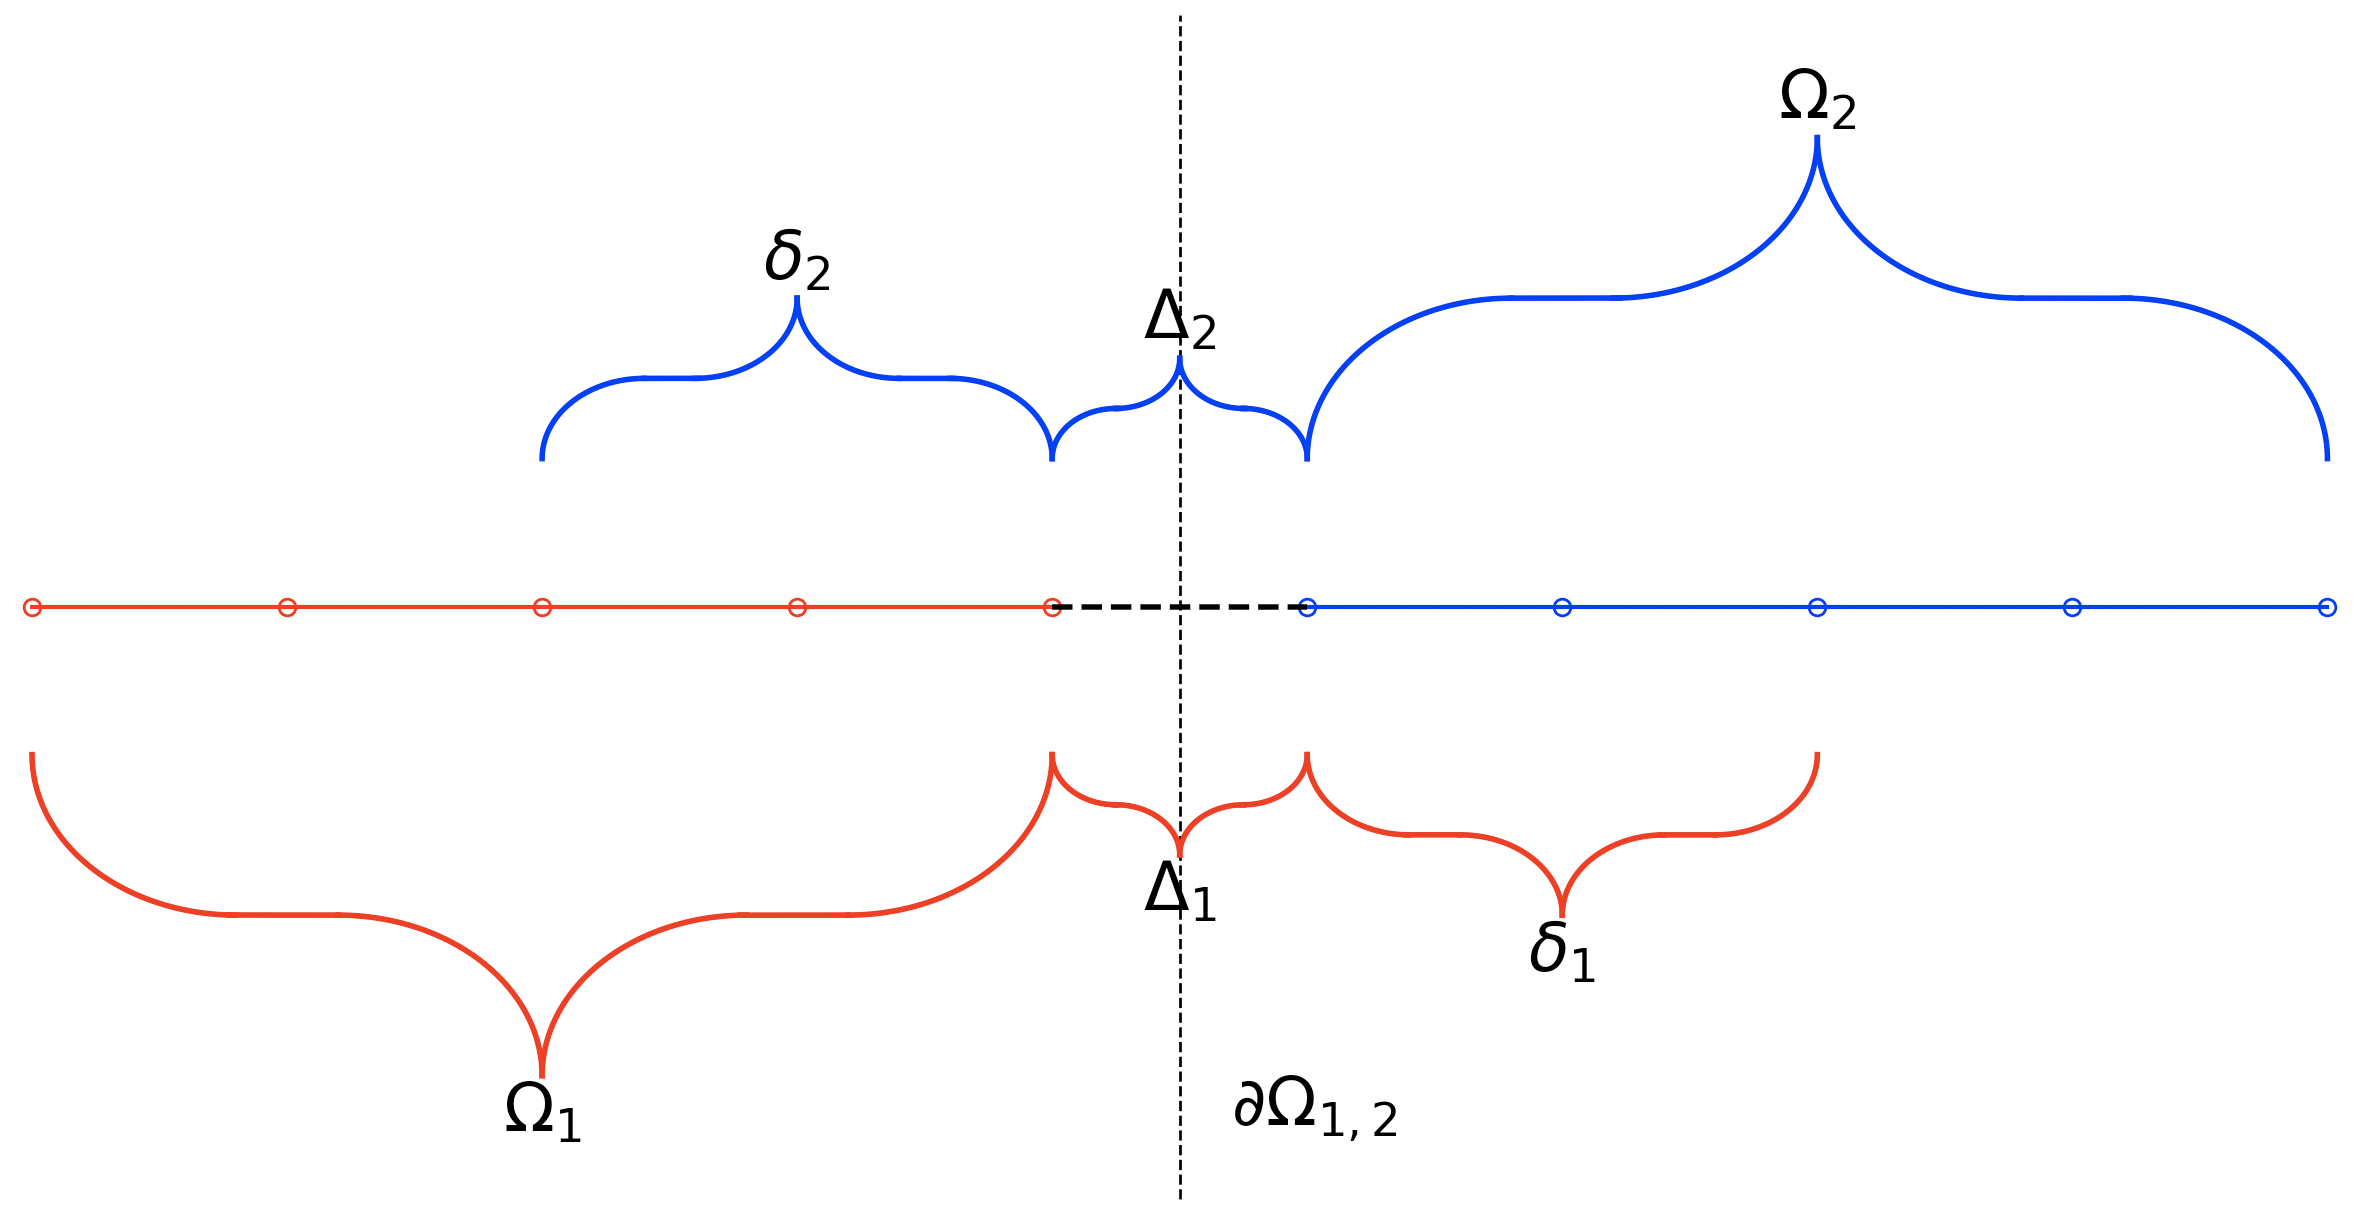
\includegraphics[width=0.47\textwidth]{figures/degree-2-1d}}
	\hfill
	\subfloat[Odd degree $p=3$\label{fig:degree-3-1d}]{%
		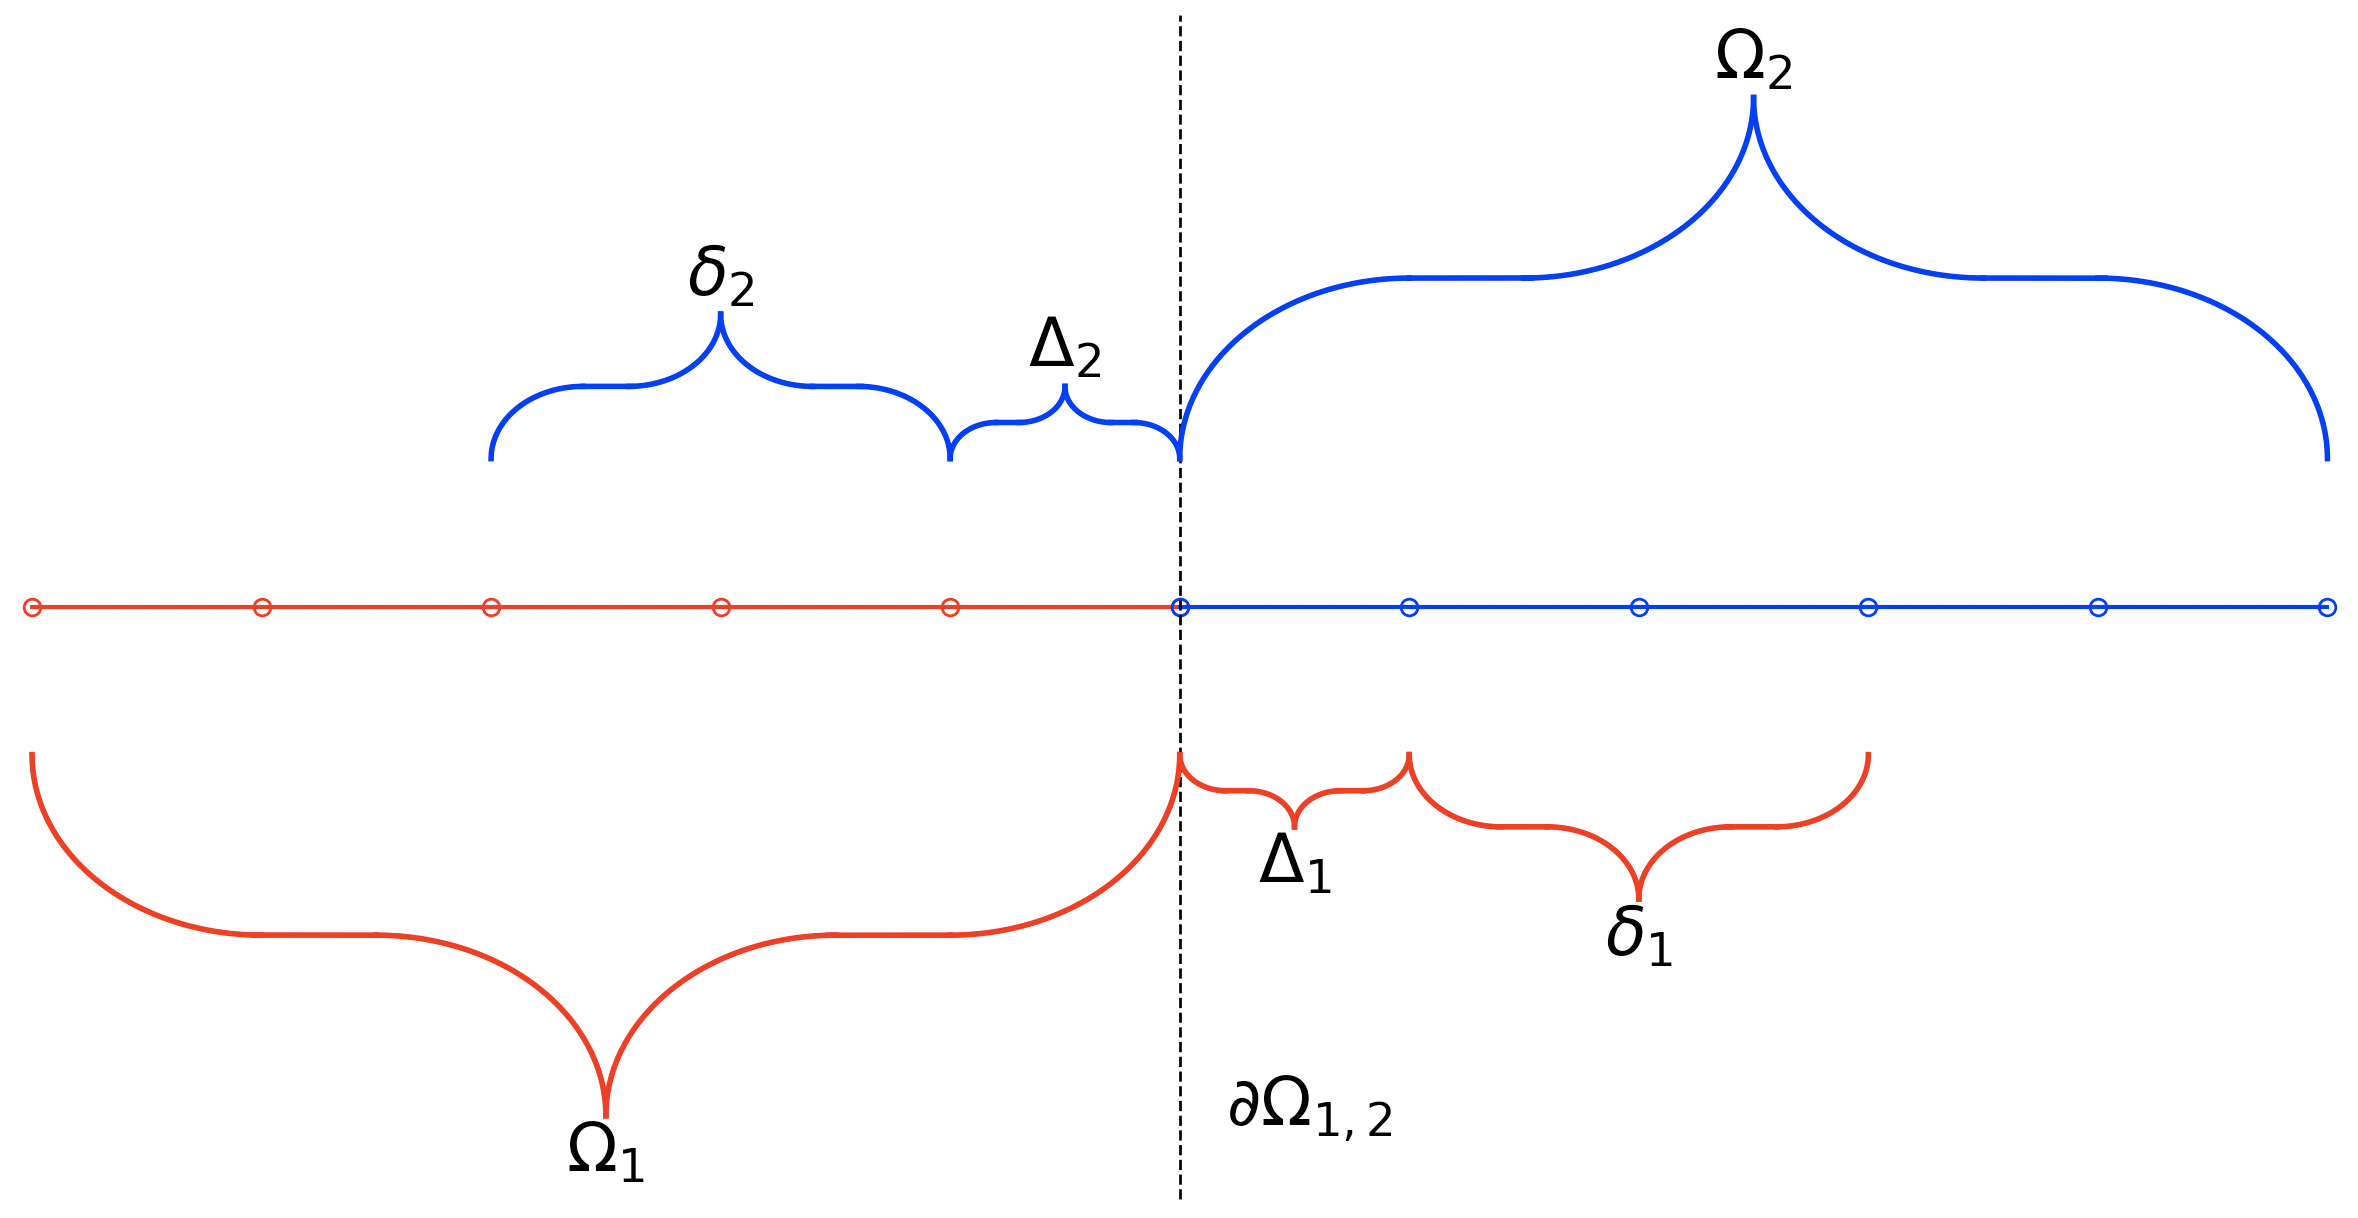
\includegraphics[width=0.47\textwidth]{figures/degree-3-1d}}
	\caption{Illustration: \dimension{1} parallel partitioned domain with floating (unclamped) interior knots and augmented spans ($\left| \delta \right|=2$)}
	\label{fig:DD-subdomain-illustration}
\end{figure}

%\comment{Talk about open vs closed?? why is open important as we try to recover single subdomain solution information. Perhaps illustrate in 1-d ?}

Instead of using clamped knots, we utilize floating (unclamped), shared knot spans near all interior subdomains such that the high-order continuity and consistency of the reconstructed solution with respect to $\mathcal{N}$ are preserved. 

For the purpose of illustration and to explain the proposed solver methodology, let us consider a simple one dimensional domain ($\Omega$) with two subdomains ($\mathcal{N}=2$) as shown in \fig{fig:DD-subdomain-illustration}, where $\Omega_1$ and $\Omega_2$ represent the subdomains that share an interface $\partial \Omega_{1,2}$. In \fig{fig:DD-subdomain-illustration}, the layout of the knot spans for both an even degree ($p=2$) and odd degree ($p=3$) are shown. For generality, we also introduce here an overlap layer $\Delta_1$ and $\Delta_2$ on each subdomain that represents the set of shared knot spans with its adjacent subdomain (for internal boundaries), and an optional augmented layer $\delta_1$ and $\delta_2$ that has a connotation similar to that of an overlap region in traditional DD schemes \cite{smith-ddm}. Note that in order to reconstruct the input data in $\Omega_i, \forall i \in [1,2]$, the knot spans must mandatorily include $\Delta_i$ regions. This $\Delta_i$ overlap region is required by definition to maintain partition of unity of a B-spline curve in order to evaluate \eqt{eq:nurbs-basis}. For generality, $\Delta_i$ represents the repeated knots along clamped global domain boundaries, and the shared knots between two subdomains in the unclamped interior boundaries.
%
For arbitrary degree $p$, the number of knot spans in $\Delta_i$ is given by $\floor{\frac{p}{2}}$, where $\floor{.}$ represents the floor operator. In multidimensional tensor product expansions, these shared spans are replaced by shared layers of knot spans along the subdomain interfaces. The $\delta_i$ regions are additional, and optional, shared knot spans that can help improve error convergence in a manner similar to overlap regions in DD methods used for PDE solvers \cite{gander-rasm, smith-ddm}. 

The control point DoF vector can be represented by three separate parts based on the local support of the basis expansion. The control point vector is in general given as $\vec{P} = [\vec{P}(\Omega); \vec{P}(\Delta); \vec{P}(\delta)]$. For the \dimension{1} scenario illustrated, this is shown below for $\mathcal{N}=2$, $p=3$ and $\left| \delta \right|=1$, where the operator $\left| \mathcal{D} \right|$ represents the number of knot spans in any underlying domain $\mathcal{D}$. 
\vspace*{-1mm}
\begin{equation}
	%\tikzset{left offset=-0.1,right offset=0.02,disable rounded corners=true}
	\tikzset{offset def/.style={
			above left offset={-0.1,0.8},
			below right offset={0.1,-0.65},
		}
	}
	\hfsetfillcolor{red!10}
	\hfsetbordercolor{red}
	%\begin{array}{@{} *{2}{ c @{} >{{}}c<{{}} @{} } c @{}}
	%16\cdot \tikzmarkin{A}I_1  & + & 11\cdot \tikzmarkin{B}I_2  & = & \tikzmarkin{C}13\\[1ex]
	%11\cdot I_1\tikzmarkend{A} & + & 16\cdot I_2\tikzmarkend{B} & = & 17\tikzmarkend{C}
	%\end{array}
	\vec{P}_1 =
	\left[
	\begin{array}{c}
		\tikzmarkin{A}(1,-0.2)(-0.1,0.3) P_1(1)   \\
		P_1 (2) \\
		\vdots   \\
		\tikzmarkend{A} P_1 (m) \\
		$\quad$ \vspace*{-2mm} \\
		\tikzmarkin{B}(0.1,-0.2)(-0.1,0.3) P_2(1) \tikzmarkend{B} \\
		$\quad$ \vspace*{-2mm} \\
		\tikzmarkin{Bp}(0.1,-0.2)(-0.1,0.3) P_2(2) \tikzmarkend{Bp} \\
		%		0 \\
		%		\vdots \\
		%		\tikzmarkend{B} 0
	\end{array}
	\right]
	, \quad \quad
	\hfsetfillcolor{blue!10}
	\hfsetbordercolor{blue}
	\vec{P}_2 =
	\left[
	\begin{array}{c}
		\tikzmarkin{D}(0.1,-0.2)(-0.1,0.3) P_2(1)   \\
		P_2 (2) \\
		\vdots   \\
		P_2 (n) \tikzmarkend{D} \\
		$\quad$ \vspace*{-2mm} \\
		\tikzmarkin{Cp}(0.1,-0.2)(-0.1,0.3) P_1(m) \tikzmarkend{Cp} \\
		$\quad$ \vspace*{-2mm} \\
		\tikzmarkin{C}(0.1,-0.2)(-0.1,0.3) P_1(m-1) \tikzmarkend{C} \\
		%		0 \\
		%		\vdots \\
		%		\tikzmarkend{D} 0
	\end{array}
	\right]
	\label{eqn:vecp-layout}
\end{equation}
%

\begin{tikzpicture}[remember picture,overlay]
	\pgfsetarrowsend{latex} 
	%
	% adjust the shift from "col" to move the position of the annotation
	\coordinate (A-aa) at ($(A)+(-0.8,-0.7)$);
	\node[align=left,left] at (A-aa) {\footnotesize{$\vec{P}_1(\Omega_1)$}};
	\path[>=stealth,red,draw] (A-aa) -- ($(A)+(0.1,-0.7)$);
	%
	% adjust the shift from "col" to move the position of the annotation
	\coordinate (B-aa) at ($(B)+(-0.8,-0.2)$);
	\node[align=left,left] at (B-aa) {\footnotesize{$\vec{P}_1(\Delta_1)$}};
	\path[>=stealth,blue,draw] (B-aa) -- ($(B)+(0.1,-0.2)$);
	%
	% adjust the shift from "col" to move the position of the annotation
	\coordinate (Bp-aa) at ($(Bp)+(-0.8,-0.2)$);
	\node[align=left,left] at (Bp-aa) {\footnotesize{$\vec{P}_1(\delta_1)$}};
	\path[>=stealth,blue,draw] (Bp-aa) -- ($(Bp)+(0.1,-0.2)$);
	%
	% adjust the shift from "col" to move the position of the annotation
	\coordinate (D-aa) at ($(D)+(2.5,-1.0)$);
	\node[align=right,right] at (D-aa) {\footnotesize{$\vec{P}_2(\Omega_2)$}};
	\path[>=stealth,blue,draw] (D-aa) -- ($(D)+(0.9,-1.0)$);
	%
	% adjust the shift from "col" to move the position of the annotation
	\coordinate (Cp-aa) at ($(Cp)+(2.5,-0.3)$);
	\node[align=right,right] at (Cp-aa) {\footnotesize{$\vec{P}_2(\Delta_2)$}};
	\path[>=stealth,red,draw] (Cp-aa) -- ($(Cp)+(1.0,-0.3)$);
	%
	% adjust the shift from "col" to move the position of the annotation
	\coordinate (C-aa) at ($(C)+(2.8,-0.3)$);
	\node[align=right,right] at (C-aa) {\footnotesize{$\vec{P}_2(\delta_2)$}};
	\path[>=stealth,red,draw] (C-aa) -- ($(C)+(1.6,-0.3)$);
	%
\end{tikzpicture}


where $m, n$ are the number of control points in $\Omega_1$ and $\Omega_2$ respectively. Note that higher degree expansions (for e.g., $p>3$) will require more support points in $\Delta$ from adjacent subdomains in order to decode the MFA up to $\partial \Omega_{1,2}$. This implies that $P_i(\Delta_i)$ in addition to the optional $P_i(\delta_i)$ vectors directly provide a measure of the required cost of communication with adjacent subdomains.

Now, the constrained minimization problem for the two subdomain case can be written as
%
\begin{equation}
	% A(X) X = F, \quad X = \left[P1 ; P2 \right]
	\left[
	\begin{array}{c|c}
		R_{1}(\Omega_1) & \lambda_{1,2}(\Delta_1 \cup \delta_1) \\
		\hline
		\lambda_{2,1}(\Delta_2 \cup \delta_2) & R_{2}(\Omega_2)
	\end{array}
	\right]
	\left[
	\begin{array}{c}
		\vec{P}_{1} \\
		\vec{P}_{2}
	\end{array}
	\right]
	=
	\left[
	\begin{array}{c}
		\vec{Q}_{1} \\
		\vec{Q}_{2}
	\end{array}
	\right]
	\label{eq:global-system}
\end{equation}

%where
%\begin{eqnarray}
%A(X) &=&
%\left[
%\begin{array}{c|c}
%A_{1,1}(P_1) & A_{1,2}(P_1,P_2^*) \\
%\hline
%A_{2,1}(P_1^*,P_2) & A_{2,2}(P_1)
%\end{array}
%\right]
%\left[
%\begin{array}{c}
%P_{1} \\
%P_{2}
%\end{array}
%\right]
%, \\ 
%&\quad& \nonumber \\
%F &=& \left[
%\begin{array}{c}
%N_1^T Q_{1} \\
%N_2^T Q_{2}
%\end{array}
%\right]
%\label{eq:coupled-operator}
%\end{eqnarray}

where the diagonal operators $R_{1}$ and $R_{2}$ are the piecewise rational functions that minimize the local subdomain residuals in $\Omega_j, \forall j \in [1,2]$, while the off-diagonal blocks $\lambda_{1,2}$ and $\lambda_{2,1}$ represent the coupling terms between the subdomains near the interface $\partial \Omega_{1,2}$. This coupling term provides the constraints on the shared control point data, and higher-order derivatives as needed to recover smoothness and enforce continuity along subdomain boundaries. For higher dimensional problems, the constraints on the control points must include both face neighbor and diagonal neighbor contributions to accurately determine the globally consistent minimization problem. 

The coupling blocks $\lambda_{i,j}$ can be viewed as Lagrange multipliers that explicitly couple the control point DoFs across a subdomain interface ($\vec{P}_{1} \cap \vec{P}_{2}$) such that continuity is preserved in a weak sense \cite{nurbs-book}. Using appropriate Schur complements to eliminate the coupled DoF contributions in each subdomain, with $\lambda_{i,j}$ evaluated at \textit{lagged} iterates of adjacent subdomains, the set of coupled constrained equations in \eqt{eq:global-system} can be completely decoupled for each subdomain. This modified system resembles a block-Jacobi operator of the global system. The scheme illustrated in this section follows ideas similar to the Jacobi-Schwarz method \cite{gander-rasm} and the overlapping,  restricted-Additive-Schwarz (RAS) scheme \cite{orasm-as-ms-2007}.
%We apply the RAS scheme to tackle this system of global equations shown in \eqt{eq:global-system}, where the coupled terms $\lambda_{i,j}$ utilize \textit{lagged} control point data from adjacent subdomains. 
%In the current paper, we instead use the Schur complement of \eqt{eq:coupled-operator} to eliminate the coupling terms by evaluating it at the lagged iterate values, in order to impose constraints in each subdomain independently. 



In the above description, the coupled data chunks, $\vec{P}_1(\Delta_1)$ and $\vec{P}_2(\Delta_2)$ belonging to adjacent subdomains near $\partial \Omega_{1,2}$ are exchanged simultaneously before the local domain solves are computed. %Since the exchanged constraint data is lagged at the previous iterate, the convergence rate in comparison to the more expensive multiplicative Schwarz variants \cite{smith-ddm} is slower.
One key advantage with such a DD scheme is that only nearest neighbor exchange of data is required, which keeps communication costs bounded as the number of subdomains $\mathcal{N}$ increase \cite{orasm-as-ms-2007, gander-rasm}, while providing opportunities to interlace recomputation of the constrained control point solution. Note that in a RAS iterative scheme, nearest neighbor exchanges can be performed compactly per dimension and direction, thereby minimizing communication costs and eliminating expensive global collectives.


\subsubsection*{Augmenting Knot Spans with Overlap}

%\subsubsection*{Constraints on Decoded Data}
%
%Instead of imposing the constraints in the control point space, alternatively, we can utilize the expansion of the MFA in input point space directly to minimize the decoded residual $E= Q - R \vec{P}$. The constraints in each subdomain then are essentially the jump terms between the decoded data on $\Omega_i$ and $\Omega_j$ shared at the interface $\partial \Omega_{i,j}$.
%
%There are some advantages to this approach compared with imposing the interface constraints in the control point space, even though the potential volume of data to be communicated between subdomains is generally much larger since it scales with size of $Q$. They are listed below.
%
%\begin{enumerate}
%	\item Subdomain residuals and boundary constraints are both in the decoded space, and hence no explicit need for a residual projection (encoding) or penalty term in \eqt{eq:nonlinear-residuals},
%	\item No explicit need for imposition of higher order derivative constraints, especially in the context of non-conforming adaptivity across subdomain interfaces, since the grid of input points is fixed,
%	\item Natural extensions within the ASM iterative scheme to generate overlapping variants.
%\end{enumerate}
%
%%Explain the iterative scheme in terms of the underlying equations and how the boundary terms are resolved through a global ASM method. First start with 1-D and talk about extensions in the scheme to allow arbitrary dimensional solver framework.
%
%When the solver is setup to use the error residuals in the actual decoded space, the natural data decomposition with overlap $\Delta$ can yield good improvements in both time and accuracy \cite{bjorstad-overlap-1989}. This follows the effectiveness of the overlapping additive-Schwarz preconditioning schemes in the context of linear algebra problems for PDEs \cite{smith-ddm} \cite{gander-rasm}. A demonstration of the improved efficiency and scalability in terms of iteration convergence is shown for a 1-D problem in the \sect{sec:results}. The growing message size for use in overlapping RAS method when solving higher dimensional problems is a concern, and it is a topic of ongoing research to find ways to minimize the communication overheads.
%
%%\begin{equation}
%%(N_i^T M_i) P_i = N_i^T T_i, \forall i \in [1, \ldots \mathcal{N}]
%%\label{eq:decoded-residuals}
%%\end{equation}


One of the key metrics of interest is that the parallel solver infrastructure does not amplify any approximation errors unresolved by the tensor product B-spline mesh. Since the local decoupled subdomain solution is encoded accurately to satisfy \eqt{eq:minimization-problem} in each individual subdomain without any data communication (i.e., embarassingly parallel), imposing the constraints for the shared DoFs in $\Delta$ should ensure the error change is bounded. However, as the control point data across subdomains become synchronized, numerical artifacts, especially for high-degree ($p>2$) basis reconstructions at subdomain interfaces can become dominant sources of error. A key metric to consider in all experiments is to validate that the multiple subdomain case produces the same error profile as a single subdomain case, in order to ensure convergence of the solvers to the same unique solution, independent of $\mathcal{N}$. %Hence, for all comparison purposes in this paper, we will consider the single subdomain solution with equivalent spatial resolution (as compared to multi-subdomain problem) to be the original reference solution. %As the number of subdomains grow, the interface errors grow proportionally, thereby generally requiring larger number of outer iterations to converge. %At convergence, we expect the overall global error in the decoded solution to be similar to the single subdomain case.


For many problem domains, overlapping variants of Schwarz solvers \cite{lions-asm, gander-rasm} have been proven to be more stable, efficient and scalable compared to nonoverlapping variants \cite{bjorstad-overlap-1989, orasm-as-ms-2007}. We utilize the concept of overlap regions by sharing additional knot spans between subdomains in order to produce better MFA reconstructions of the underlying data. This user-specified, additional overlap is described by $\delta_j, \forall j \in [1,2]$ in \fig{fig:DD-subdomain-illustration}. The amount of data overlap utilized for computing the functional approximation can directly affect the conditioning in the subdomain solver, and the scalability of the overall algorithm. Additionally, we expect the residual errors $\vec{E}$ from the approximation to remain bounded as the number of subdomain increase with appropriate overlap regions. %And the overall accuracy of the parallel algorithm cannot be worse than the single subdomain case.

For better clarity, we will use overlap regions $\delta$, as illustrated in \fig{fig:2d-schematic} for a \dimension{2} problem with $p=3$ and $\mathcal{N}=4$, to increase the size of the local problem ($\Omega$), and to improve the accuracy of domain decomposed approximations. We note that the control point data $\vec{P}$ in both the $\Delta$ and $\delta$ overlap regions are shared and uniformly weighted (averaged) by $\vec{P}$ computed in the neighboring subdomains.

Note that in the \dimension{2} schematic, shared data in $\delta$ regions are always exchanged between neighboring subdomains. The set of $\vec{P}(\delta)$ are explicitly used only to impose constraints that contribute to the reconstruction of datasets, and hence play a role in the approximation error of MFA. It is also important to note that when $\vec{P}$ DoFs are {\em multishared} between subdomains, then shared data between multiple $\Omega_j, \forall j \in [0,3]$ need to be exchanged in order to compute $\vec{P}_i(\delta_i), \forall i \in [0,3]$.


%\comment{Talk about exchanging additional knot spans in addition to the required support required for unclamped interior subdomain solution}



\begin{figure}[htbp]
	\centering
	\begin{tikzpicture}
		\begin{scope}[xshift=1.5cm]
			\node[anchor=south west,inner sep=0] (image) at (0,0) {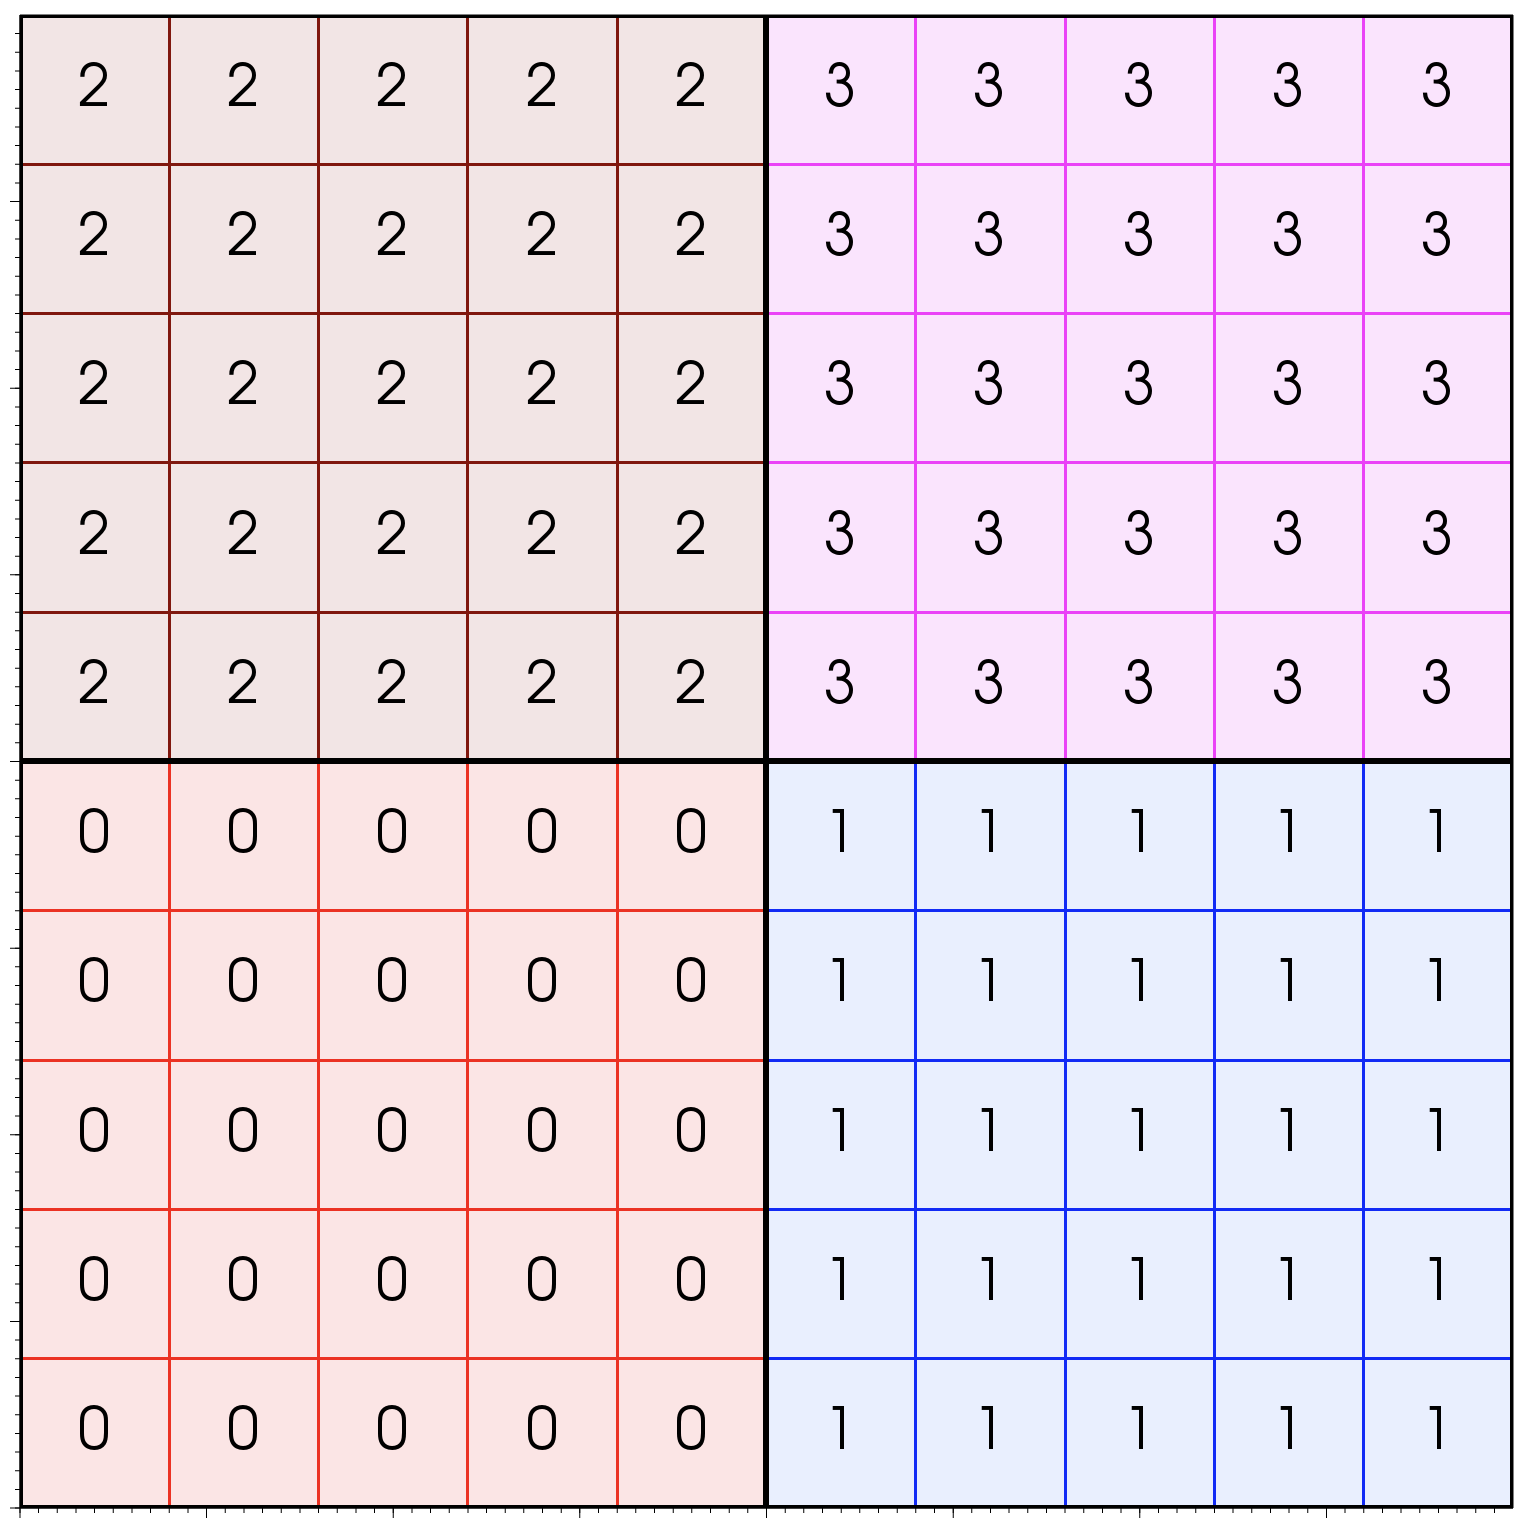
\includegraphics[width=0.44\textwidth]{figures/2d-schematic-4subd.png}};
			\begin{scope}[x={(image.south east)},y={(image.north west)}]
				\draw[black,ultra thick,rounded corners] (0.49,0.0) rectangle (0.61,0.61);
				\draw[black,ultra thick,rounded corners] (0.0,0.49) rectangle (0.61,0.61);
				\draw[black,ultra thick,densely dashed,rounded corners] (0.59,0.0) rectangle (0.71,0.71);
				\draw[black,ultra thick,densely dashed,rounded corners] (0.0,0.59) rectangle (0.71,0.71);
				\draw[black,ultra thick,dotted,rounded corners] (0.0,0.0) rectangle (0.51,0.51);
				
				\draw[red,ultra thick,rounded corners] (0.29,0.29) rectangle (0.71,0.71);
				\node[draw] at (-0.07, 0.25) {\large $\Omega_0$};
				\node[draw] at (-0.07, 0.55) {\large $\Delta_0$};
				\node[draw] at (-0.07, 0.66) {\large $\delta_0$};
				\node[draw] at (0.55,-0.07) {\large $\Delta_0$};
				\node[draw] at (0.66,-0.07) {\large $\delta_0$};
				
				%\draw [-latex, ultra thick, red] (note) to[out=0, in=-120] (0.48,0.80);
				\draw [-stealth, line width=2pt, red] (0.71,0.5) -- (1.1,0.5);
				\node[draw] at (1.35,0.5) {multishared region};
			\end{scope}
			%	\centering
			%	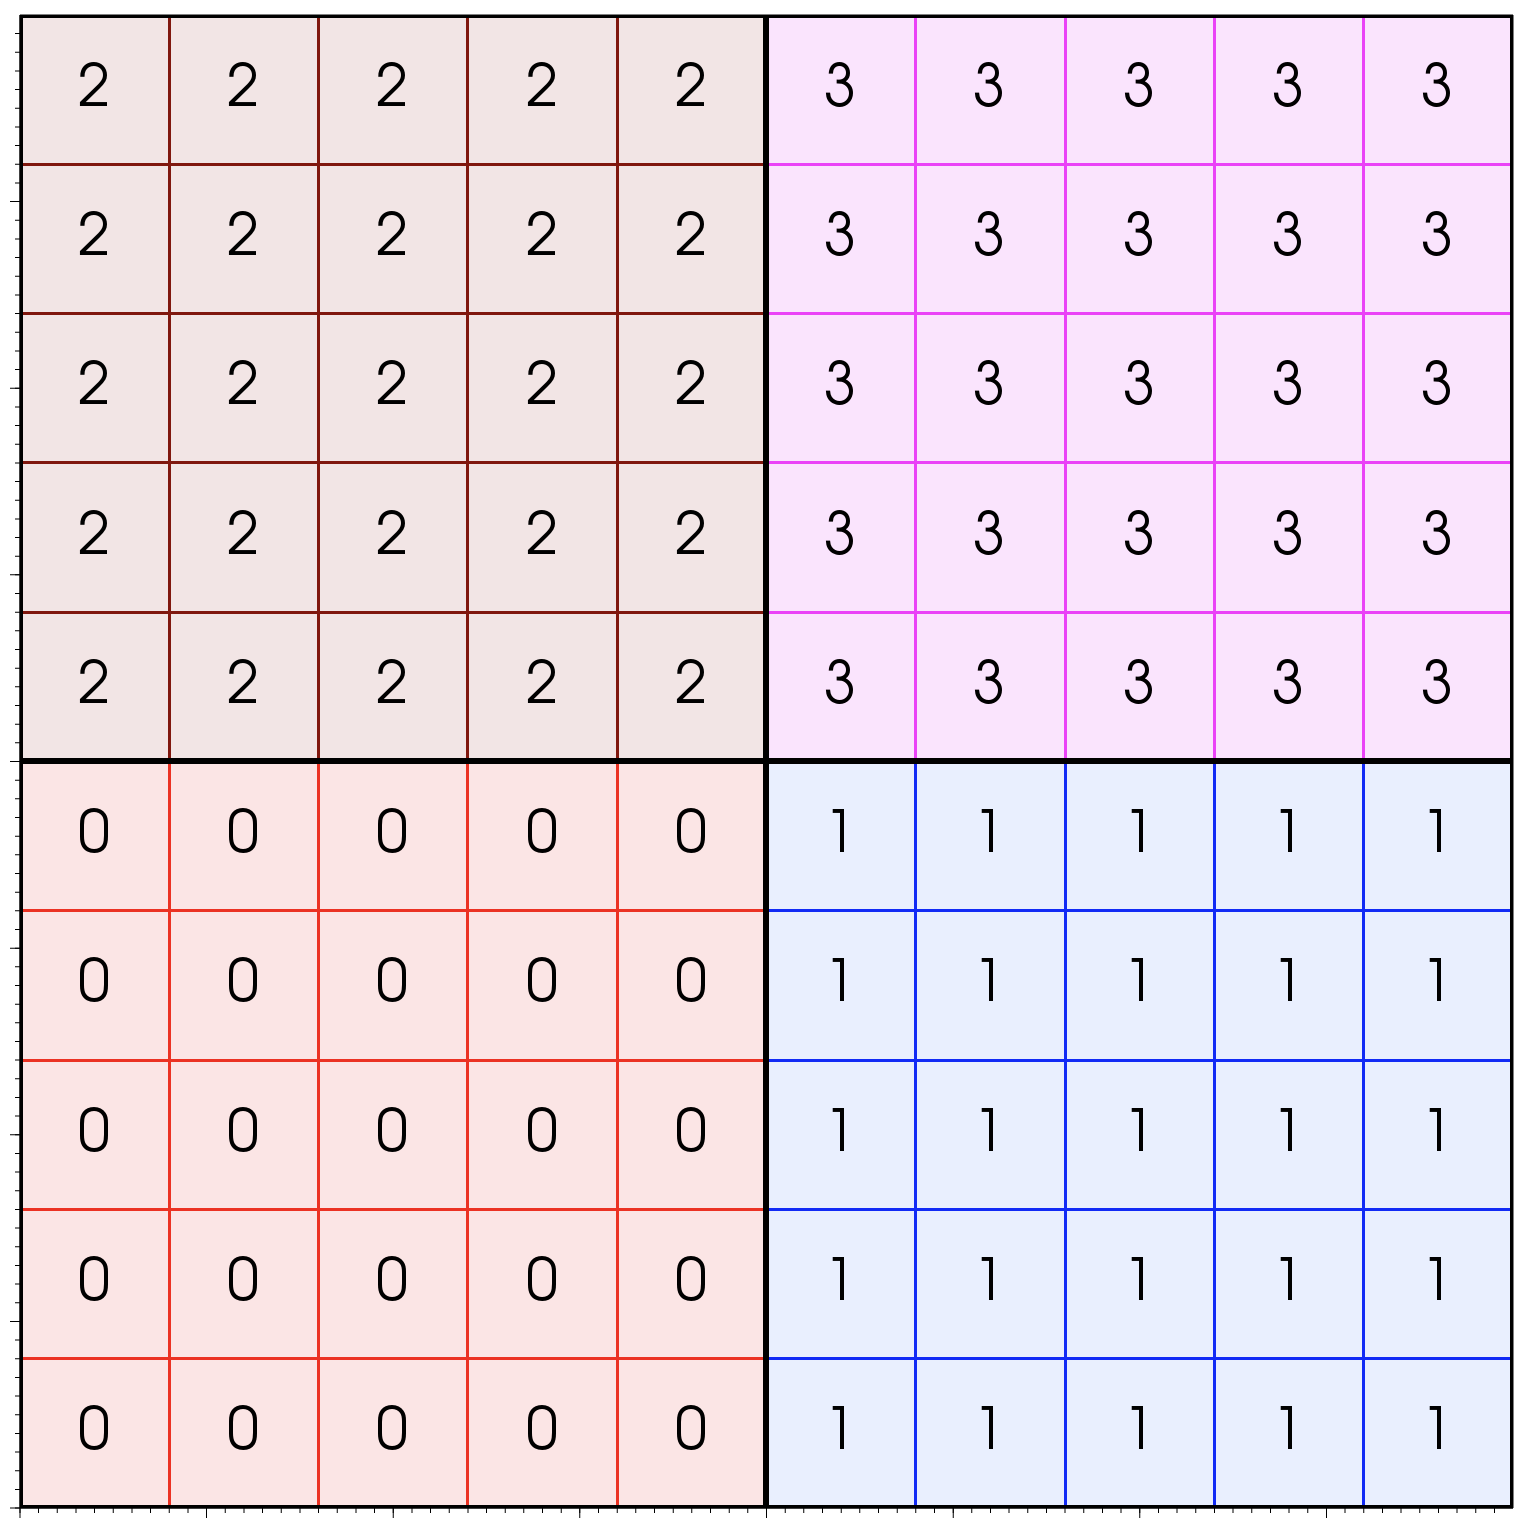
\includegraphics[width=0.45\textwidth]{figures/2d-schematic-4subd.png}
			
		\end{scope}
	\end{tikzpicture}%
	\caption{\dimension{2} subdomains with $\mathcal{N}=4$, $p=3$ and the augmented overlap $\left| \delta \right|=1$ showing local subdomains $\Omega_i$, mandatory overlap for floating knots $\Delta_i$, optional overlap regions $\delta_i$, where $i \in [0,\mathcal{N}-1]$, and multishared DoF regions that couple multiple subdomains (marked in red).}
	\label{fig:2d-schematic}
\end{figure}



%\subsection{Constrained Linear Least-Squares Solver}
%
%Given the user specification to obtain a $C^0, C^1$ or $C^2$ continuity across block interfaces, the local subdomain solve can essentially be formulated as the solution to a LSQ problem with constraints. The idea here is to introduce additional unknowns in the solutions, which are essentially the Lagrange multipliers to obtain an augmented system of equations.
%
%If we consider the local system introduced in \eqt{eq:LSQ-system}, the solution $P$ is the unconstrained control point data that is only piecewise continuous globally. Then, we can introduce a constrained set of equations \cite{nurbs-book} such that 
%
%\begin{equation}
%(N_i^T M_i) P_i = N_i^T T_i, \forall i \in [1, \ldots \mathcal{N}]
%\label{eq:LSQ-system-constraint}
%\end{equation}
%
%where $M$ is the basis matrix corresponding to the constrained DoFs and $T$ is the vector of input data in the overlap region of interest $\Delta$. Then the constrained linear least squares curve fitting problem is simply minimizing the residual $E=Q-RP$ such that $MP=T$ is satisfied. We refer the readers to Section (9.4.2) in \cite{nurbs-book} for further details on how a Schur complement of the coupled equation systems can be applied to eliminate the Lagrange multipliers in order to enforce the constraints within each subdomain system. This particular strategy can also be extended to higher dimensions easily with larger number of constraints included in the $M$ operator.


We also introduce a definition for compression ratio ($\eta$), which gives the ratio of the total input points in the dataset ($dim\text{ }\vec{Q}$) to the total control points ($dim\text{ }\vec{P}$) used in the MFA B-spline representation. As $\eta \rightarrow 1$, one can achieve better error residuals in comparison to the reference data for a given degree $p$, while $\eta \gg 1$ produces smooth approximations with larger error profiles. When we analyze the results in this manuscript, it should be remembered that the reconstruction error is always inversely proportional to $\eta$.

Next, the parallel MFA computation workflow that will be used with domain-decomposed subdomain partitions is presented in detail. 

\subsection{Solver Workflow}
\label{sec:solver-methodology}

Computing the functional approximation to large-scale datasets requires efficient solvers at two levels: firstly, the local decoupled subdomain solver for  \eqt{eq:minimization-problem}, and next, the constrained minimization problem in \eqt{eq:global-constrained-problem}. Hence, the global problem reduces to a series of local minimization problems in each subdomain.

%
\begin{equation}
	\begin{aligned}
		% Scalar miniization problem
		%r_i(\Omega_i) &=& \left\lVert Q_i - R_i \vec{P}_i \right\rVert_2, \quad \forall i \in [1, \mathcal{N}] \nonumber \\
		%r_c(\Delta_{i})    &=& \sum_{j \in \partial \Omega_i} \left\lVert \vec{P}_i(\Delta_i) - \vec{P}_{j}(\Omega_{j} \cap \Delta_{i} )  \right\rVert_2 \nonumber \\ 
		%r_i(\Omega_i \bigcup \Delta_{i}) &=&  r_i(\Omega_i) + \epsilon r_c(\Delta_{i}), 
		% Vector minimization problem
		%\vec{E}_i(\Omega_i) &=& Q_{\ell} - R_{\ell} \vec{P}_{\ell}, \quad \forall {\ell} \in \Omega_i \nonumber \\
		%\vec{E}_c(\Delta_{i})    &=& \sum_{\partial \Omega_{i,j}} \left[ \mathcal{F}( \vec{P}_{i}(\Delta_i \cap \Omega_{j}) )  \right] \nonumber \\ 
		%
		& \argmin_{\vec{P} \in \mathbb{R}^n} & & \left\lVert \vec{Q}_{\ell} - R_{\ell} \vec{P}_{\ell} \right\rVert_{L_2}, \quad R_{\ell} \in \mathbb{R}^{m \times n}, \vec{Q}_{\ell} \in \mathbb{R}^m, \vec{P}_{\ell} \in \Omega_i \\
		%
		& \text{subject to} & & \sum_{\partial \Omega_{i,j}} \left[ \mathcal{F}_{ij}( \vec{P}_{i}(\Delta_i), \vec{P}_{j}(\Omega_j) )  + \mathcal{F}_{ij}( \vec{P}_{i}(\delta_i), \vec{P}_{j}(\Omega_j) )  \right]^2 = 0, \quad \forall i, j \in [1,\ldots\mathcal{N}]
		%
		%\vec{E}_c(\Delta_{i})    &=& \sum_{\partial \Omega_{i,j}} \left[ \mathcal{F}_{ij}( \vec{P}_{i}(\Delta_i) )  \right] \nonumber \\ 
		%\vec{E}_i(\Omega_i \bigcup \Delta_{i}) &=&  \vec{E}_i(\Omega_i) + \epsilon \vec{E}_c(\Delta_{i}), 
		\label{eq:nonlinear-residuals}
	\end{aligned}
\end{equation}

where $\Omega_j$ are the neighboring subdomains of $\Omega_i$, $\mathcal{F}_{ij}(a,b)$ is the jump term across the shared interface DoFs $a$ and $b$ defined on subdomains $i$ and $j$ respectively. 
%In our experiments, a large value of $\epsilon=10^{7}$ has yielded very good performance with favorably monotonic error reduction in the constraint residuals $r_c(\Delta_{i})$. Note that $\vec{E}_i(\Omega_i)$ is in the decoded space, while the constraint residual $\vec{E}_c(\Delta_{i})$ is in the control point space. Hence in this formulation, we apply the constraints directly on control points, while trying to minimize the overall decoding error for the MFA within the current subdomain thereby satisfying optimality in terms of local resolution and continuity preservation at boundaries.


\subsubsection{Subdomain Solvers}

For the linear LSQ solvers that can be used to compute local subdomain control point solution $\vec{P}$, there are a variety of choices available. Direct methods like Singular Value decomposition or Cholesky decomposition operating on the normal equations \cite{bjorck1996} can compute optimal values. Alternatively, the iterative LSQ solvers such as orthogonal decomposition methods based on QR and QZ factorizations are more stable, especially when the normal form of the operator, $R^T R$, is ill-conditioned. %\cite{zheng-bo-bspline-bfgs}

\subsubsection{Restricted Additive-Schwarz Solvers}

The outer RAS iterations work together with nearest neighbor communication procedures to exchange shared DoF data between adjacent subdomains. This is an important step to ensure that $\vec{P}$ data computed through the LSQ procedure are consistent and high-order continuous across subdomain boundaries. The final minimized control point solution is achieved when the interface solutions match on all $\partial \Omega_{i,j} \in \Omega$ rendering zero jump residuals ($\mathcal{F}_{ij}$) on $\Delta$ and $\delta$ shared domains in \eqt{eq:nonlinear-residuals}.

%\todo{Imposing Linear Constraints on Shared DoFs: Illustrate in \dimension{1} case, how the shared DoFs are handled. Split between an even and odd case. Odd case is specifically constraints in the even case, in addition to a weighted average constraint on the interface control point DoF}

%\comment{Compute subdomain solutions independently for the problem using Eq 1;
	%Then exchange nearest neighbor data and impose constraints;
	%re-solve the problem and converge shared data}


%In order to ensure continuity across NURBS patches, Zhang et al.  \cite{zhang-nurbs-continuity} evaluated the constraint matrix at test points along the interface curve. These computations require a Singular Value Decomposition (SVD) solve at every interface and can become prohibitively expensive as dimensionality increases. Alternatively, we can use a nonlinear minimizer, directly applied to the system in \eqt{eq:global-system}, and adding a penalty term to the constrained DoFs represented by the coupling blocks $\lambda_{i,j}$. Such a system can be expressed as a minimization problem in each subdomain with the following objective functional.


%The augmented solution on each local subdomain after nearest neighbor exchange contains only the control points and corresponding derivative data to constrain DoFs on both the left and right interfaces in 1-D. This definition extends naturally to higher dimensions, with the penalized constraints on the boundary terms evaluated as a loop over all shared interfaces to compute the net residual. 

%To compute the solution to the minimization problem in \eqt{eq:nonlinear-residuals}, we can make use of Sequential Least SQuares Programming (SLSQP) solver with equality constraints, or apply the limited memory version of  Broyden-Fletcher-Goldfarb-Shannon ($\ell$-BFGS) algorithm when the dimensionality increases, and memory requirements become large. These solvers have already been proven effective for converging such constrained continuity problems with B-Splines \cite{zheng-bo-bspline-bfgs}. 
%An even more efficient method is to reformulate the objective function as a root finding problem, and applying Krylov accelerators or Anderson mixing to compute the optimally constrained solutions, with much lower computational complexity and superior convergence properties. However, these approaches have not been explored here. 
%The final minimized control point solution is achieved when the interface solutions match on all $\partial \Omega_{i,j} \in \Omega$ rendering zero jump residuals ($\mathcal{F}_{ij}$) on $\Delta$ and $\delta$ shared domains in \eqt{eq:nonlinear-residuals}.

%A much more efficient solver would also be to use a Krylov accelerator for the subdomain solves, which expresses the components in \eqt{eq:nonlinear-residuals} as a vector to reformulate it as a root finding problem. In our experiments, the Krylov accelerator was typically much faster to converge and compute the optimally constrained solutions.

It is also important to note that unlike the blending approaches that can be directly applied on decoded data \cite{grindeanu-blending}, the numerical error with the constrained iterative scheme is not bounded by the original partitioned, unconstrained least-squares solution; i,e., imposing subdomain boundary constraints can create artificial numerical peaks (non-monotonic) in reconstructed data as we converge towards continuity recovery. A solution to address this issue is to increase the amount of overlap range to ensure uniform convergence to the true single-subdomain solution error, even as the number of subdomains ($\mathcal{N}$) increases.


%\subsubsection*{Convergence of RAS}

The nonoverlapping and overlapping RAS scheme applied to the computation of MFA exhibits scalable convergence properties in the limit of decreasing subdomain size (i.e., as $\mathcal{N} \to \infty$). This is a favorable property for strong scaling, especially when tackling large datasets, as the net computational cost always remains bounded. This behavior can be explained by the nature of how the RAS iterative procedure resolves the shared DoFs.

By using a weighted averaging procedure for all shared DoFs that reside in the $\Delta$ and $\delta$ domains, each outer iteration resolves any disparity in $\vec{P}$. The DoFs values on shared vertices ($d > 0$), edges ($d > 1$) and faces ($d > 2$) are resolved in the following order in consequent RAS iterations.
%
\begin{enumerate}
	\item Singly-shared ($\mathcal{SS}$) DoFs that are shared between two adjacent, neighboring subdomains; e.g., direct interface data belonging to $(\Delta_i \cup \delta_i) \cap \Omega_j$ in \fig{fig:2d-schematic}, $\forall i \in [1, \mathcal{N}]$ and $j \in [1, \hat{\mathcal{N}}]$, where $\hat{\mathcal{N}}$ represents the set of nearest neighbors sharing an interface $\Omega_{i,j}$
	\item Multi-shared ($\mathcal{MS}$) DoFs that are shared by multiple (more than 2) neighboring subdomains; e.g., diagonal corners that result from $\mathcal{S}_0 \cap \mathcal{S}_1 \cap \mathcal{S}_2 \cap \mathcal{S}_3$ in \fig{fig:2d-schematic}, where $\mathcal{S}_i=\Omega_i\cup\Delta_i\cup\delta_i$.
\end{enumerate}
%
Given both these specific DoF groups, the overlapping RAS scheme applied to MFA computation {\em always converges in 2 outer iterations} for problems in \dimension{2} and \dimension{3}, and a single iteration in \dimension{1} (due to lack of $\mathcal{MS}$ DoFs). This result is demonstrated in \sect{sec:results}. Note that achieving full convergence with high-order continuity in a single iteration is possible by combining constraints for both $\mathcal{SS}$ and $\mathcal{MS}$ DoFs. However, due to complexities in the implementation of constraint matching in \eqt{eq:nonlinear-residuals} for this algorithmic optimization, it has not been pursued here.% \comment{demonstrate in results section}

It is necessary to mention that we use a uniform weighting procedure to converge the shared DoFs between different subdomains, where the weights for each shared DoF is assigned as $w_i=\frac{1}{n_s}$, with $n_s$ being the number of subdomains containing DoF $i$ within its domain $\mathcal{S}$. This weighing procedure can be trivially replaced by Shephard's functions, especially in the context of adaptive discretizations with variable knot displacements.

%\todo{Explain that the convergence of RAS strictly depends on the dimensionality of the problem i.e., for a given spatial dimension, the number of iterations to converge to a final solution with $C^p$ continuity is always fixed (independent of $n$ and $p$). For \dimension{1}, the iterations converge in 2 iterations, for \dimension{2} in 3 iterations and \dimension{3} in 4 iterations. This can be explained by the nature of how the shared DoFs are converged through linear constraints at every iterate. Provide an illustration in \dimension{3} how the errorchange converges to zero with first error getting resolved on vertices, then edges and faces.}




\subsubsection{Note on Performance Characteristics}


%
%Once the interface constraint data terms are received, a Schur complement of \eqt{eq:coupled-operator} can be computed to eliminate the coupling terms, and to impose constraints in each subdomain independently. This leads to an augmented subdomain solution as shown in \eqt{eq:augmented-solution} that includes the control point, and optionally the derivative and weights at the interface obtained from the adjacent subdomain. 
%
%It is imperative to note that the only exchange of data between subdomains is performed through nearest neighbor communication that has bounded complexity and costs. 
The volume of messages exchanged between subdomains depends on several computational factors.

\begin{enumerate}
	\item \textbf{Clamping}: If the boundary knots are pinned, or if they have a floating knot description at subdomain interfaces depending on whether $C^0$ or $C^{p-1}$ continuity is required,
	\item \textbf{Parity}: Whether the MFA degree of expansion is odd or even, which determines the range of common knot spans shared between adjacent domains as given by $\Delta$ (refer to \fig{fig:DD-subdomain-illustration}),
	%\item \textbf{Continuity}: The degree of continuity (up to $p-1$) determines the stencil needed to enforce the constraints on either side of the interface 
	\item \textbf{Overlap}: The amount of augmented overlap ($\delta$), which determines the number of additional coupled data layers to be communicated between neighboring domains, both in terms of the input span space $\vec{Q}$, and control point DoFs $\vec{P}$ (refer to \fig{fig:DD-subdomain-illustration} and \fig{fig:2d-schematic}).
\end{enumerate}

At convergence, the interface data at $\partial \Omega_{1,2}$ will satisfy the higher-order continuity prescriptions specified by the user, thereby guaranteeing full regularity of $C^{p-1}$. The illustration in \fig{fig:DD-subdomain-illustration}, and the methodology description in this section can be generalized and extended to arbitrary dimensions in the tensor-product setting (with the parametric domain represented by a $d-$dimensional hypercube) as shown in \fig{fig:2d-schematic} for \dimension{2}. Using knot insertion and removal strategies based on deCasteljau subdivision procedures \cite{nurbs-book}, individual subdomains can also be adapted to resolve fast varying solutions and to reduce decoded error to be within user-specified tolerances \cite{nashed-rational}. While adaptivity has not been fully explored in the current work, enabling variable resolutions in different dimensions is a natural extension of the work that will still preserve high-order continuity.
The implementation of the presented approach with domain decomposition strategies, combined with overlapping RAS scheme yields a scalable scheme that will be demonstrated to be suitable for tackling large-scale data analysis problems.

\subsection{Implementation}
\label{sec:implementation}

%
% \begin{algorithm}
	% 	% \DontPrintSemicolon
	% 	\KwData{Input dataset and coordinates}
	% 	\KwData{Parameters: $\mathcal{N}, p$}
	% 	\tcp*{decompose domain into blocks with DIY}
	% 	\tcp*{solve local LSQ problem without constraints}
	% 	\tcp*[h]{Outer RAS loop;}\;
	% 	\While{ converged == False }
	% 	{
		% 		$\vec{P}(\Omega \cap \Delta)$ $\rightarrow$ enqueue outgoing constraints\;
		% 		exchange constraints with nearest neighbor blocks\;
		% 		$\vec{P}(\Delta)$ $\leftarrow$ dequeue incoming constraints\;
		% 		\tcp*[h]{Inner $\ell$-BFGS/Krylov minimization solver}\;
		% %		\For {$isub \in \mathcal{N}$}
		%		 {
			% 			$\vec{P}_i \leftarrow$ solve adaptive local MFA with constraints\;
			% 			$E_i \leftarrow$ compute decoded local error\;
			% 			$\delta \vec{P} (\Omega_i) \leftarrow \vec{P}_{iASM} (\Omega_i) - \vec{P}_{iASM-1} (\Omega_i)$\;
			% 		}
		% 		dPMax $\leftarrow \left\lVert \delta \vec{P} (\Omega_i) \right\rVert_{\infty}$\;
		% 		iASM++\;
		% 	}
	% 	\tcp*[h]{Store subdomain solution data;}\;
	%    Write MFA to disk for analysis and visualization
	%
	%
	% \end{algorithm}


\begin{algorithm}
	\caption{Domain Decomposed MFA Solver}
	\label{alg:pseudocode}
	\begin{algorithmic}
		\State{\textbf{Input:} Dataset and coordinates}
		\State{\textbf{Parameters:} $\mathcal{N}, p, m$}
		\State{\textbf{Setup:} Decompose domain into blocks with DIY, compute $R$}
		\While{$\vec{P}(\Omega)$ not converged}
		\For{$i \gets 1$ to $\mathcal{N}$}
		\If{$\vec{P}_i = 0$}
			\State{\textbf{Solve:} Unconstrained local LSQ problem}
		\EndIf
		\For{$j \gets 1$ to $\mathcal{\hat{N}}$}
		\Comment{where $\mathcal{\hat{N}}$ = nearest neighbors}
		\State{-- $\vec{P}_i(\Omega_i \cap (\Delta_j \cup \delta_j)) \rightarrow$ enqueue outgoing constraints}
		\State{-- Exchange shared DoFs with all nearest neighbor blocks}
		\State{-- $\vec{P}_i(\Delta_i \cup \delta_i)$ $\leftarrow$ dequeue incoming constraints}
		%
%		\State{-- Enforce constraints for $\vec{P}_i(\Delta_i \cup \delta_i) \cap \vec{P}_j, \forall j \in [1, \mathcal{N}]$ as illustrated in \eqt{eqn:vecp-layout}}
%		%
%		\State{-- Drive $\mathcal{F}_{ij} \rightarrow 0$ for all shared DoFs in $\Delta_i \cup \delta_i$}
		%
		\State{-- Enforce constraints for $\vec{P}_i(\Delta_i \cup \delta_i) \cap \vec{P}_j, \forall j \in [1, \mathcal{N}]$:  Drive $\mathcal{F}_{ij} \rightarrow 0$}
		\EndFor
		
		\State{-- Update local error $E_i := \left\lVert \vec{Q}_i - R \vec{P}_i \right\rVert_{L_2} $}
		
		\EndFor

		\State{Check convergence metrics}
		
		\EndWhile
		\State{Write MFA to disk for analysis and visualization}
	\end{algorithmic}
\end{algorithm}

The DD techniques presented here for MFA computation are primarily implemented in Python, with main dependencies on \texttt{SciPy} for B-spline bases evaluations and linear algebra routines. Additionally, the drivers utilize Python bindings (\texttt{PyDIY}) for the \texttt{DIY}~\cite{morozov16} C++ library. \texttt{DIY} is a programming model and runtime
for block-parallel analytics on distributed-memory machines, built on \texttt{MPI-3}~\cite{dongarra13}.  Rather than programming
for process parallelism directly in \texttt{MPI}, the programming model in \texttt{DIY} is based on block parallelism. In \texttt{DIY}, data are decomposed
into subdomains called blocks. One or more of these blocks are assigned to processing elements (processes or threads) and the computation is
described over these blocks, and communication between blocks is defined by reusable patterns. 
%The same \texttt{DIY} program consisting of a block-parallel decomposition can be run on different numbers of \texttt{MPI} processes and it is the responsibility of the \texttt{DIY} runtime to map between blocks and processes. 
\texttt{PyDIY} utilizes \texttt{PyBind11}~\cite{jakob17} and \texttt{MPI4Py}~\cite{dalcin11} to expose the interfaces in the C++ library. In our implementation, \texttt{PyDIY} is exclusively used to manage the data decomposition, including specifications to share an interface $\partial \Omega_{i,j}$ and ghost layers that represent the $\Delta \cup  \delta$ overlapping domains.

The overall approach is sketched in \algo{alg:pseudocode}.
% \Remark{Vijay: finish the pseudocode and expand the discussion of it below.} 
We begin by decomposing the domain into a set of regular blocks aligned with the principal axes
of the global domain. Before enforcing constraints, the local subdomain solves are performed completely decoupled so that the discontinuous MFA to represent the partitioned input data is computed. %We also include adaptive knot placements to approximate the input data by introducing control point DoFs where needed to capture solution data variations. 
%
The control point solution from this decoupled LSQ problem solver is then used as the DoF data that needs to be constrained with RAS iterative method.
We then begin iterating over the blocks to converge the shared DoFs through the linear constraints described in \sect{sec:solver-methodology}. 

At the start of each iteration, the control point constraints are exchanged between neighboring blocks in a regular nearest-neighbor communication pattern. This is sufficient to update the constraints $\vec{P}(\Delta \cup \delta)$. \texttt{DIY} 
%\texttt{enqueue} and \texttt{dequeue} data exchange API 
sends and receives the constraint data to neighboring blocks based on the parallel data decomposition.
The nonlinear residual error in each subdomain is a function of the tensor product mesh resolution and degree $p$. At convergence, we expect to recover the subdomain error that is identical to the single subdomain case.
%Depending on whether the MFA residual or the decoded residual norms are to be minimized, a subdomain solver is chosen to drive the nonlinear residual for the local block within user-specified tolerances.

%At the end of the outer iterative loop, we check for convergence across all subdomains, by evaluating whether the maxima of the $L_{\infty}$ error across all subdomains ($\mathcal{N}$) of the ASM update vector is within user-specified tolerance. If this condition is satisfied, the MFA computation is stopped.
The final result, as described in \algo{alg:pseudocode}, is a global MFA that retains high-order continuity and accuracy of a single subdomain solve, but with excellent parallel efficiency to reduce total time to solution as the number of subdomains increases.

%\Remark{\algo{alg:pseudocode} is just a skeleton. Details need to be filled in. Termination conditions, local (inner loop) iterative scheme, types of constraints (control points or decoded points), etc.}


%\begin{equation}
%	%\tikzset{left offset=-0.1,right offset=0.02,disable rounded corners=true}
%	\tikzset{offset def/.style={
		%			above left offset={-0.1,0.8},
		%			below right offset={0.1,-0.65},
		%		}
	%	}
%	\hfsetfillcolor{blue!10}
%	\hfsetbordercolor{blue}
%	%\begin{array}{@{} *{2}{ c @{} >{{}}c<{{}} @{} } c @{}}
%	%16\cdot \tikzmarkin{A}I_1  & + & 11\cdot \tikzmarkin{B}I_2  & = & \tikzmarkin{C}13\\[1ex]
%	%11\cdot I_1\tikzmarkend{A} & + & 16\cdot I_2\tikzmarkend{B} & = & 17\tikzmarkend{C}
%	%\end{array}
%	P_1^{'} =
%	\left[
%	\begin{array}{c}
	%		\tikzmarkin{A}(1,-0.3)(-0.1,0.3) P_1(1)   \\
	%		P_1 (2) \\
	%		\vdots   \\
	%		\tikzmarkend{A} P_1 (m) \\
	%		$\quad$ \vspace*{-2mm} \\
	%		\tikzmarkin{B}(0.6,-0.1)(-0.1,0.3) P_2(1) \\
	%		0 \\
	%		\vdots \\
	%		\tikzmarkend{B} 0
	%	\end{array}
%	\right]
%	,
%	\hfsetfillcolor{red!10}
%	\hfsetbordercolor{red}
%	P_2^{'} =
%	\left[
%	\begin{array}{c}
	%		\tikzmarkin{C}(1,-0.3)(-0.1,0.3) P_2(1)   \\
	%		P_2 (2) \\
	%		\vdots   \\
	%		\tikzmarkend{C} P_2 (n) \\
	%		$\quad$ \vspace*{-2mm} \\
	%		\tikzmarkin{D}(0.6,-0.1)(-0.1,0.3) P_1(1) \\
	%		0 \\
	%		\vdots \\
	%		\tikzmarkend{D} 0
	%	\end{array}
%	\right]
%	\label{eq:augmented-solution}
%\end{equation}
%%
%\begin{tikzpicture}[remember picture,overlay]
%	\pgfsetarrowsend{latex} 
%	%
%	% adjust the shift from "col" to move the position of the annotation
%	\coordinate (A-aa) at ($(A)+(-0.5,-1.0)$);
%	\node[align=left,left] at (A-aa) {\footnotesize{$P_1$($\Omega_1$)}};
%	\path[>=stealth,blue,draw] (A-aa) -- ($(A)+(0.2,-1.0)$);
%	%
%	% adjust the shift from "col" to move the position of the annotation
%	\coordinate (B-aa) at ($(B)+(-0.5,-1.0)$);
%	\node[align=left,left] at (B-aa) {\footnotesize{$P_1$($\Delta_1$)}};
%	\path[>=stealth,blue,draw] (B-aa) -- ($(B)+(0.2,-1.0)$);
%	%
%	% adjust the shift from "col" to move the position of the annotation
%	\coordinate (C-aa) at ($(C)+(1.4,-1.0)$);
%	\node[align=right,right] at (C-aa) {\footnotesize{$P_2$($\Omega_2$)}};
%	\path[>=stealth,red,draw] (C-aa) -- ($(C)+(0.75,-1.0)$);
%	%
%	% adjust the shift from "col" to move the position of the annotation
%	\coordinate (D-aa) at ($(D)+(1.4,-1.0)$);
%	\node[align=right,right] at (D-aa) {\footnotesize{$P_2$($\Delta_2$)}};
%	\path[>=stealth,red,draw] (D-aa) -- ($(D)+(0.75,-1.0)$);
%	%
%\end{tikzpicture}
%



%% Results section

\section{Results}
\label{sec:results}

To demonstrate the effectiveness of the nested iterative algorithm, we utilize both analytical closed form functionals and scientific datasets in both 1-D and 2-D obtained from high-fidelity simulations. A brief description of the problem cases that are used as test datasets is given below.

\begin{enumerate}
	\item Synthetic data: sinc($x$)=$\frac{sin(x)}{x}$ functional on $\Omega \in [-4, 4]$
	\begin{itemize}
		\item 1-D: Q(x) = sinc($x$) + sinc(2$x$-1) + sinc(3$x$+1.5), 
		% z = scale * ( np.sinc((X+1)**2 + (Y-1)**2) + np.sinc(((X-1)**2 + (Y+1)**2)) )
		\item 2-D: Q(x,y) = sinc($(x+1)^2+(y-1)^2$) + sinc($(x-1)^2+(y+1)^2$)
	\end{itemize}
%	\item Nek5000: A 3-D dataset from CFD simulation with velocity magnitude as the solution profile
	\item S3D: A 3-D turbulent combustion dataset generated by an S3D simulation \cite{chen-s3d-2009} of fuel jet combustion in the presence of an external cross-flow. 
	\item CESM: A 2-D Community Atmosphere Model climate model dataset on a sphere with 3600x1800 resolution
\end{enumerate}


\subsection{1-D Results}\label{AA}

%\begin{itemize}
%	\item Use the first two problems to measure convergence in parallel as number of domains increase
%	\item Talk about adaptivity and resolution of data even for highly varying problem data.
%\end{itemize}

\subsubsection{Adaptive Error Convergence and Verification}

The 1-D implementation of the ASM iterative solver was applied to the analytical sinc problem. An initial input problem size of 500 points was evaluated as a test case, and MFA representation for the resulting profile was computed on 4 subdomains. The solution profile, along with the control point locations from the adaptive computation are shown in \fig{fig:sinc-adaptive-a}. We utilized the residual definition shown in \eqt{eq:nonlinear-residuals} with a $G_1$ constraint to be satisfied along all internal subdomain interfaces. The \fig{fig:sinc-adaptive-b} and \fig{fig:sinc-adaptive-c} present the zoomed in reconstruction of the approximation near the interface between $\Omega_2$ and $\Omega_3$ before, and after the ASM iterations are converged. The initially discontinuous solutions from independent, adaptive, unconstrained subdomain solves are converged to satisfy the constraints after only 3 RAS iterations, with nearest neighbor exchange of control point data at the interfaces to recover $G_1$ continuity.

\begin{figure}
	\centering
	\subfloat[sinc function profile in 1-D\label{fig:sinc-adaptive-a}]{%
		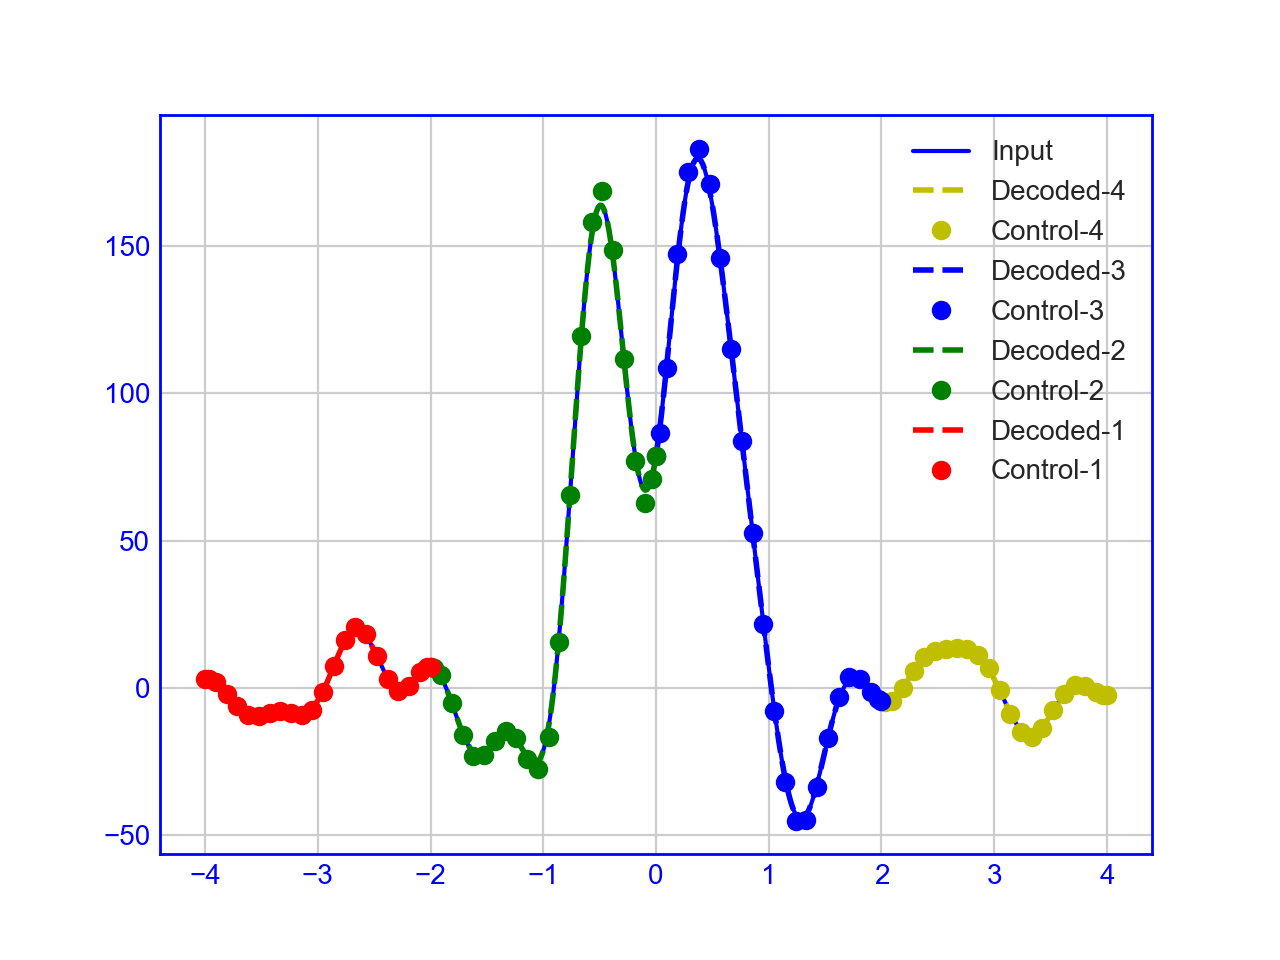
\includegraphics[width=0.5\textwidth]{figures/sinc-1d-profile}}
	\hfill
	\subfloat[Zoomed in image of $\Omega_{2,3}$ at (a) iASM=0\label{fig:sinc-adaptive-b}]{%
		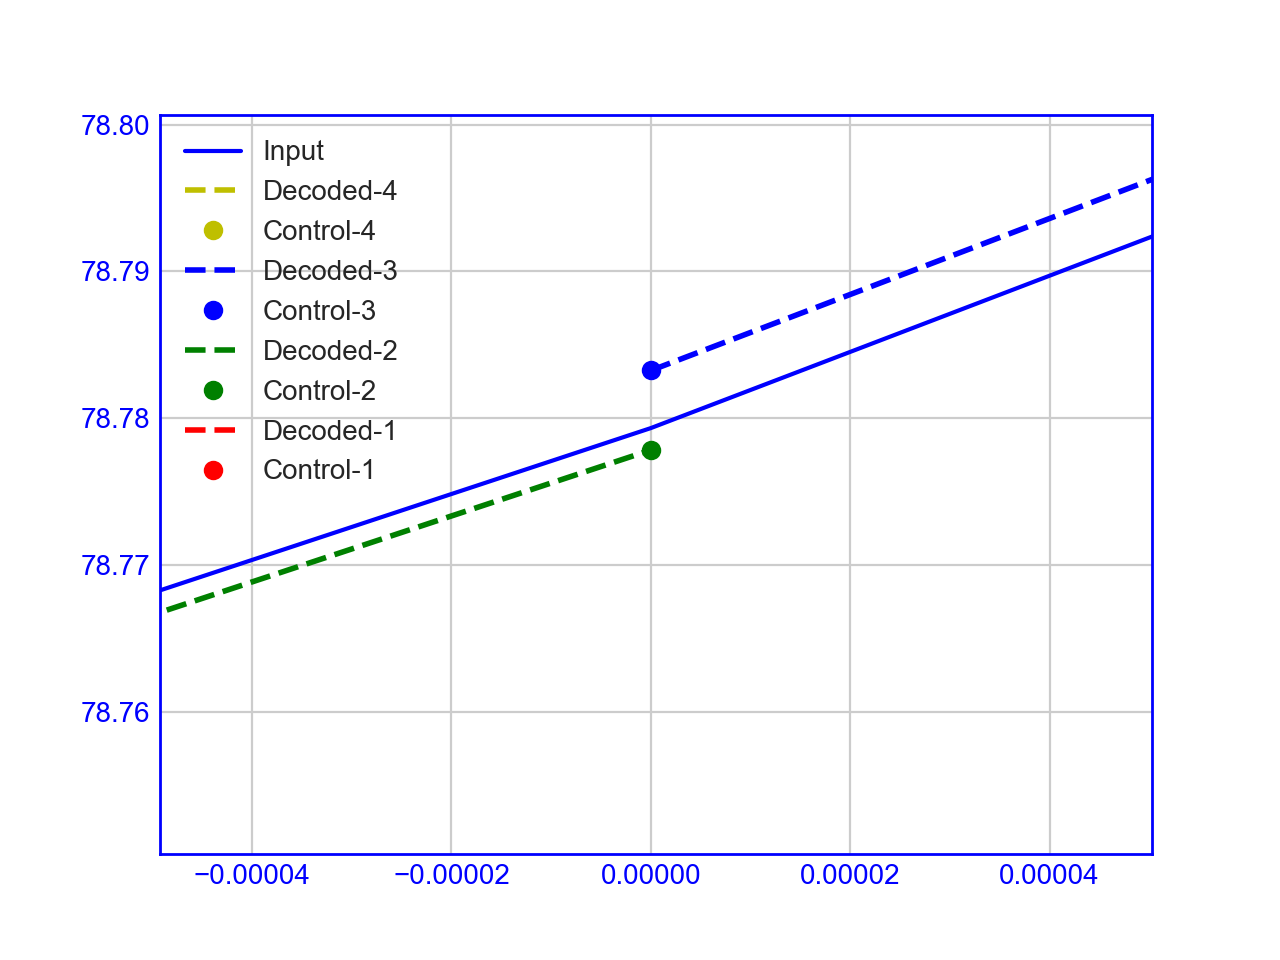
\includegraphics[width=0.5\textwidth]{figures/sinc-1d-discontinuous}}
	\\
	\subfloat[Zoomed in images of $\Omega_{2,3}$ at iASM=3\label{fig:sinc-adaptive-c}]{%
		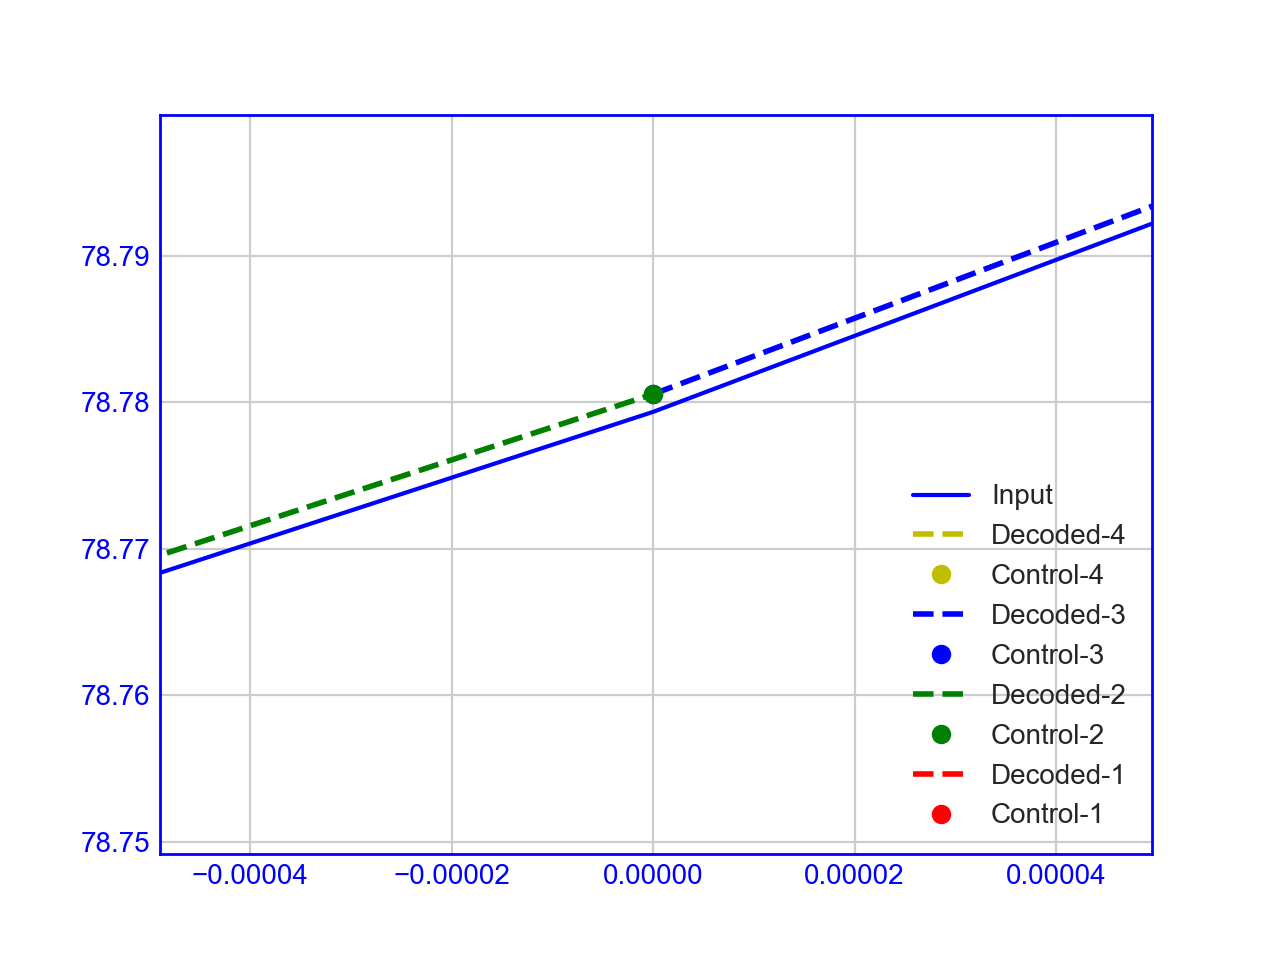
\includegraphics[width=0.5\textwidth]{figures/sinc-1d-continuous}}
	\caption{1-D analytical sinc dataset with 501 input points: adaptive MFA on 4 subdomains with $10^{-4}$ 	tolerance and $p=2$}
	\label{fig:sinc-adaptive}
\end{figure}

%\subsubsection{Subdomain Solver Performance}
%
%Compare LCLSQ - Encoded nonlinear and Decoded nonlinear

\subsubsection{Overlap Experiments in 1-D}

In this 1-D experiment on the closed form sinc function shown in \sect{sec:results}, we utilize the decoded residual minimization with the RAS-Krylov solver combination, and increase the amount of overlap in the input points to look at the convergence speed of the RAS method. We measured the global $L_2$ error convergence along with the total cost in terms of outer iteration to compute the constrained control point locations. In this analysis, adaptivity in the individual subdomains was explicitly turned off so as to maintain a constant ratio of input points to control points per subdomain, as overlap region is extended in the subdomains on both the left and right sides.

\fig{fig:decoded-overlap-data-performance} shows the global $L_2$ norm of the net error in the decoded residual, as the number of subdomains are increased. With no overlap regions, where only the interface data is shared, the total ASM iterations needed to satisfy convergence, and the net error increases linearly with $n_s$. As the overlap size becomes larger, for $\Delta=32$ and $\Delta=64$, the error growth and the number of iterations to achieve convergence remain much more bounded in comparison with the non-overlapping case. The implications of this particular result closely matches the ASM preconditioning theory often applied in PDE solvers \cite{smith-ddm, lions-asm, gander-rasm}. It also shows that the RAS iterative scheme can be accelerated more efficiently, and scalably as a solver without a prohibitive linear complexity of O($n_s$).

\begin{figure}
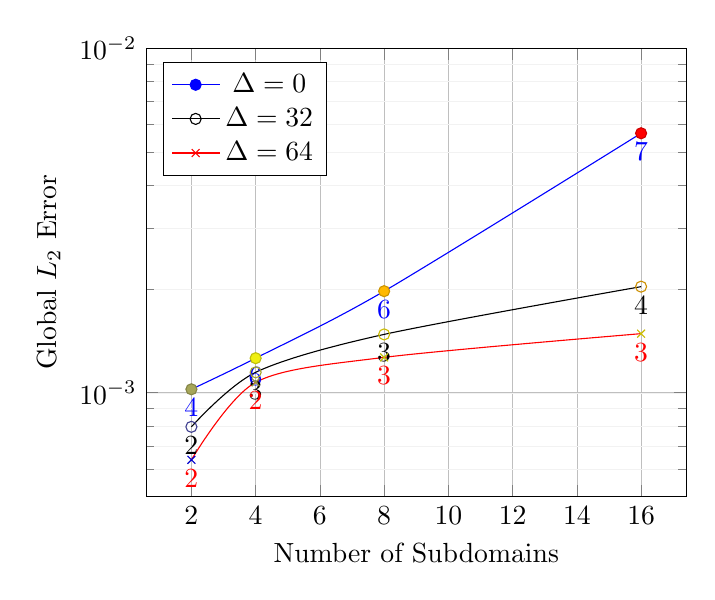
\begin{tikzpicture}

\begin{semilogyaxis}[
legend pos= north west,
ymin = 0.0005, ymax = 0.01,
xlabel=Number of Subdomains,
ylabel=Global $L_2$ Error,
nodes near coords*={\Label},
visualization depends on={value \thisrow{label} \as \Label},
grid=both,
grid style={line width=.1pt, draw=gray!10},
major grid style={line width=.2pt,draw=gray!50},
axis line style={latex-latex},
%axis lines=middle,
]
\axispath\draw
(7.49165,-10.02171)
|-  (8.31801,-11.32467)
node[near start,left] {$\frac{dy}{dx} = -2.58$};

\addplot[smooth,mark=*,blue] table [meta=class]  {
	x y class label
	2    0.001023481 A 4
	4    0.001259901 B 6
	8    0.001971792 C 6
	16   0.005663382 D 7
};

\addplot[smooth,mark=o,black] table [meta=class]  {
	x y class label
	2    0.000796565 A 2
	4    0.001146259 B 3
	8    0.001477074 C 3
	16   0.002032123 D 4
};

\addplot[smooth,mark=x,red] table [meta=class]  {
	x y class label
	2    0.000638741 A 2
	4    0.001072061 B 2
	8    0.001266798 C 3
	16   0.001484362 D 3
};

%\addplot[smooth,mark=*,blue] plot coordinates {
%	(2,    0.001023481)
%	(4,    0.001259901)
%	(8,    0.001971792)
%	(16,   0.005663382)
%};

%\addplot[smooth,mark=o,black] plot coordinates {
%	(2,    0.000796565)
%	(4,    0.001146259)
%	(8,    0.001477074)
%	(16,   0.002032123)
%};

%\addplot[smooth,mark=x,red] plot coordinates {
%	(2,    0.000638741)
%	(4,    0.001072061)
%	(8,    0.001266798)
%	(16,   0.001484362)
%};

\legend{$\Delta=0$\\$\Delta=32$\\$\Delta=64$\\}

\end{semilogyaxis}
\end{tikzpicture}
\caption{1-D sinc problem with 1025 points: Accuracy convergence and number of iterations of ASM solver with overlap variations, as $n_s$ increases}
\label{fig:decoded-overlap-data-performance}
\end{figure}

\subsection{2-D Results}

Using the 2-D sinc analytical function, the error convergence for different NURBS bases degree $p$ was measured. As the number of control point DoFs are increased, the global norm of the errors are reduced consistently in the current implementation. Next we tested the spatial adaptivity in 2-D on a scientific dataset to ensure that the hierarchical iterative scheme with RAS is able to capture strong solution variations, and still ensure continuity across subdomain interfaces. 
%Using varying fidelity of the real world data, and the ability to create complex closed form functionals within our Python implementation, the approach was verification for accuracy using uniform control point refinements to yield sizes theoretical convergence orders. 
%We utilize the described 2-D problem datasets to better understand the convergence and parallel scalability of the proposed algorithms at scale. Demonstrations for the S3D, and CESM datasets are provided below.

\subsubsection{S3D Dataset: Spatial Adaptivity}

Additionally, using adaptive resolution based on a-posteriori gradient estimates, numerical errors in strongly varying solution profiles were reduced to within user-specified tolerances. A sample solution for the 2-D slice of the S3D dataset on 9 subdomains is shown in \fig{fig:s3d-adaptive-2d}, along with the error profiles at the first iteration in \fig{fig:s3d-adaptive-2d-b} and on convergence of the RAS iterations in {fig:s3d-adaptive-2d-c}.

\begin{figure}
	\centering
	\subfloat[S3D dataset profile\label{fig:s3d-adaptive-2d-a}]{%
	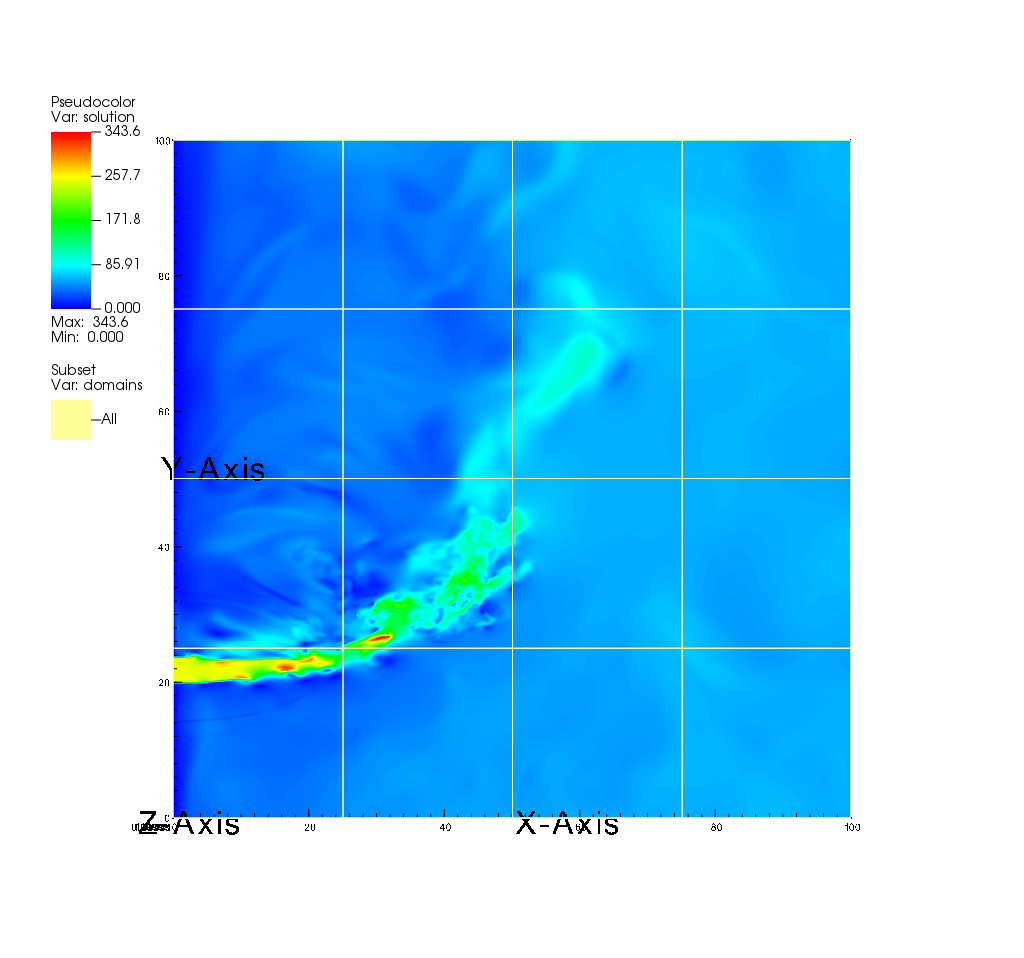
\includegraphics[width=0.44\textwidth]{figures/s3d-2d-profile.png}}
	\hfill
	\subfloat[Error profile before RAS iteration or adaptivity\label{fig:s3d-adaptive-2d-b}]{%
		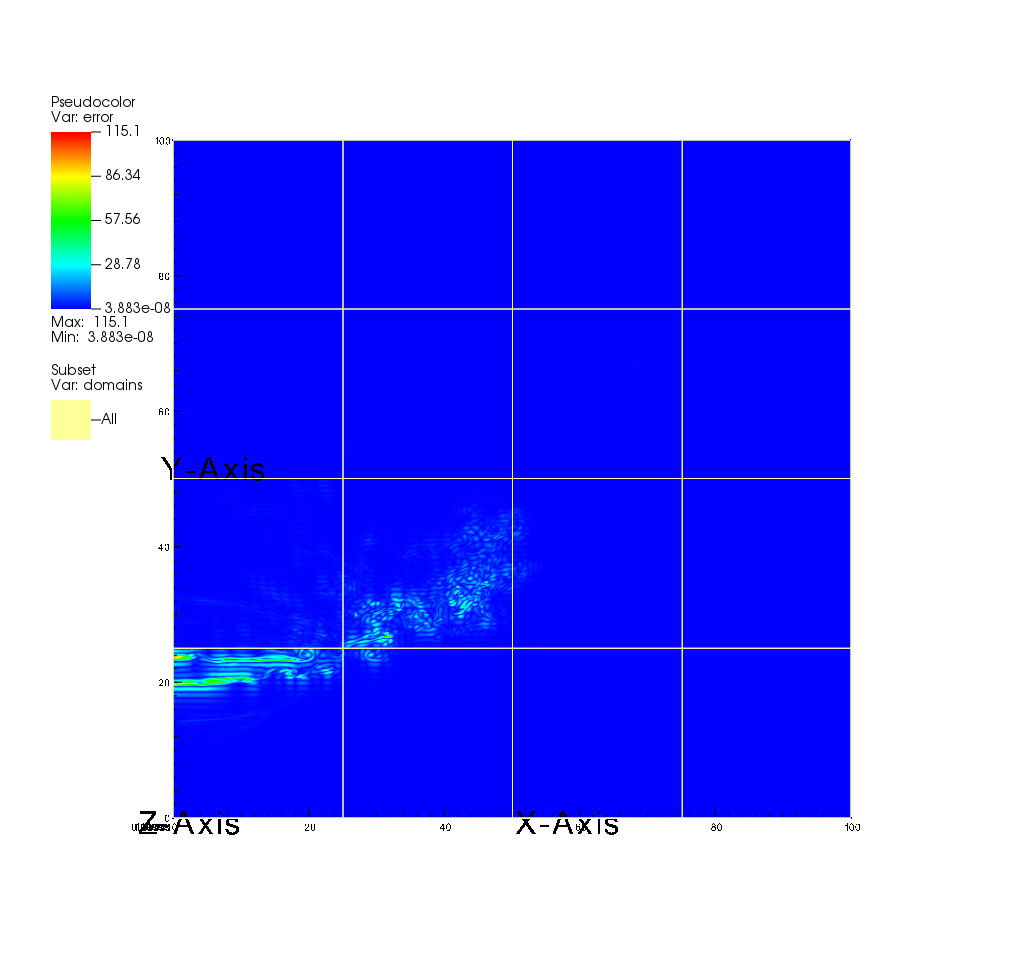
\includegraphics[width=0.44\textwidth]{figures/s3d-error-iter1}}\\
	\subfloat[Error profile after RAS iteration converges\label{fig:s3d-adaptive-2d-c}]{%
		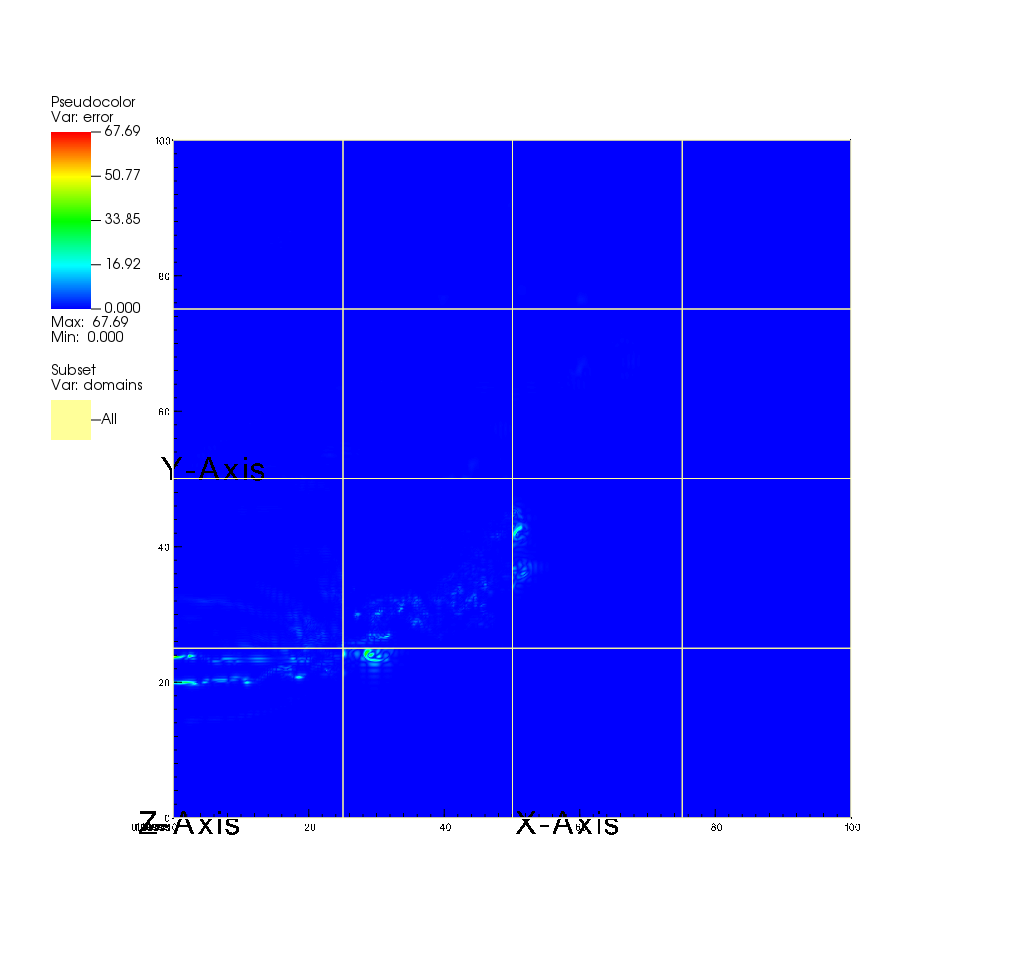
\includegraphics[width=0.44\textwidth]{figures/s3d-error-iter4}}
	\caption{2-D slice of the S3D dataset: profile and adaptive error resolution with tolerance=$10^{-2}$}
	\label{fig:s3d-adaptive-2d}
\end{figure}

The errors in the decoupled LSQ solve shown in \fig{fig:s3d-adaptive-2d-b} has relatively larger errors in the subdomains with strong gradient changes. When including knot adaptivity combined with RAS iterative scheme, the errors in the reconstructed MFA data are reduced to within user-specified relative tolerances of $10^{-2}$. This result demonstrates the convergence of the proposed scheme to adaptively resolve a complex scientific solution profile, even on a small number of subdomains ($n_s=16$). 

%\Remark{show error convergence plots for S3D on 16 subdomains with adaptivity}

%that even with the coarse resolution with 16 subdomains, 

%\subsubsection{Nek5000 dataset}
%
%\Remark{add table of actual compression and error as $n_s$ is changed}

%\Remark{Discuss about complications and potential ways to enforce continuity. (a) Use decoded data, (b) Use control point space across interface}


\subsubsection{Parallel Scalability}\label{sec:parallel-scalability}

The parallel scalability of the implemented RAS iterative solver for ensuring continuity across block boundaries was measured on the 2-D CESM dataset, whose solution profile in a uniform latitude-longitude grid is shown in \fig{fig:cesm-2d-profile}. 
Our experiments were executed on the Bebop cluster at
Argonne National Laboratory LCRC (Laboratory Computing Resource Center). Bebop has 1024 public nodes, with Intel Broadwell or Intel Knights Landing processors, with 128 GB memory per Broadwell node, and 104 GB per KNL node. It has an Omni-Path Fabric Interconnect. Broadwell processors have 36 cores, while KNL processors have 64 cores. We primarily used the KNL processors for the scalability tests presented below.

A strong scalability test was performed on the Bebop cluster with the CESM dataset, using 32 subdomains in the X-direction and 128 subdomains in the Y-direction. With this fixed DD and a uniformly placed, 100 control points per subdomain (10x10) resolution, parallel jobs were executed to compute the MFA. The Python driver utilized DIY to handle block decompositions and rank assignment, as the total number of processes used in the parallel run was varied from [1,2,$\ldots$2048]. We measured the overall time for the initial subdomain solves, and the consequent RAS iteration cycle for $nMaxASM=5$. The time to compute the MFA in parallel is shown for this strong scalability experiment in \fig{fig:cesm-strong-scalability}.

\begin{figure}
	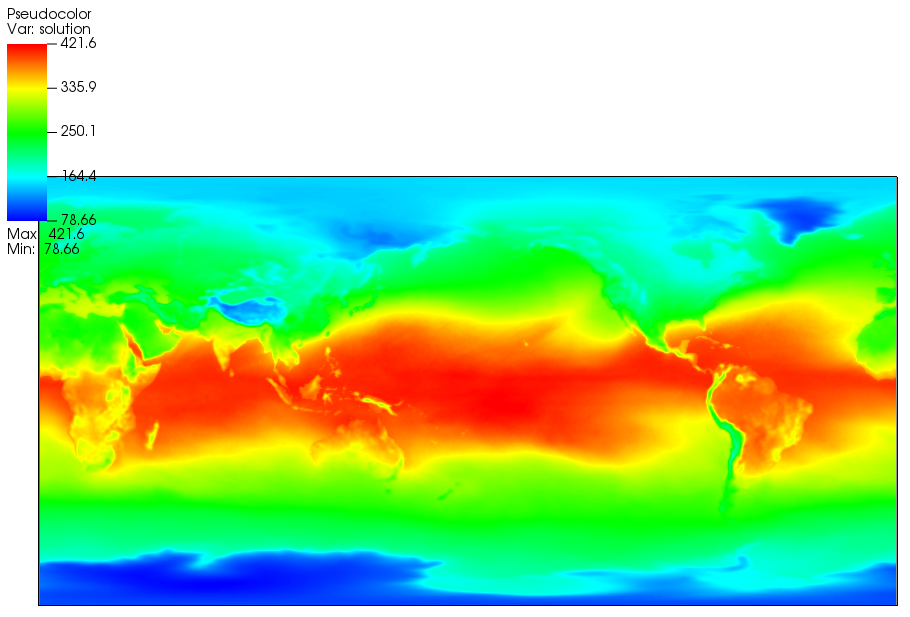
\includegraphics[width=0.45\textwidth]{figures/cesm-profile.png}
	\caption{2-D CESM climate dataset}
	\label{fig:cesm-2d-profile}
\end{figure}

As expected, the hierarchical iterative scheme with RAS-Krylov combination shows excellent scalability for the chosen dataset, and the overall time to compute the MFA was reduced from nearly 7000s on a single process, to 9.5s on 2,048 processes, while ensuring both $G_0$, and $G_1$ continuity in the domain interfaces. The ratio of computational work in local subdomain solves in comparison with communication time in nearest-neighbor exchanges gradually increases as subdomain size shrinks. This is due to the fact that global information on smaller subdomains take multiple iterations to propagate, and hence using overlaps for such large problems would be a recommended extension in the future to improve overall scalability of the algorithm. For this intermediate size problem, the strong scaling efficiency of the presented scheme is around 35\% on 2,048 processes, which dropped off from 65\% parallel efficiency at 256 processes.

Another key verification performed during this strong scaling test is to ensure that the local subdomain errors computed in serial and on different process counts remain the same at convergence. This verification is important to reiterate the fact that the approximation error due to the constrained solves to recover higher-order continuity does not significantly affect the error metrics for the MFA.

%\Remark{should we try to do a performance model for this particular case ?
%	communication: C = 4096*4 = 16384 messages
%	serial = 5C + 5A
%	parallel = 5C + 5A/p
%}

%CESM dataset has 6.5M data points
%We used 32*128 = 4096 subdomains for the strong scaling test
%\Remark{How does the nearest neighbor communication stay bounded ? measure timings separately ?}

%jobrun_neup cesm_p1 1 1 python ../Projection-2D.py -x 32 -y 128 -p 5 -c 10 -a 5 --disableadaptivity 

\begin{figure}
	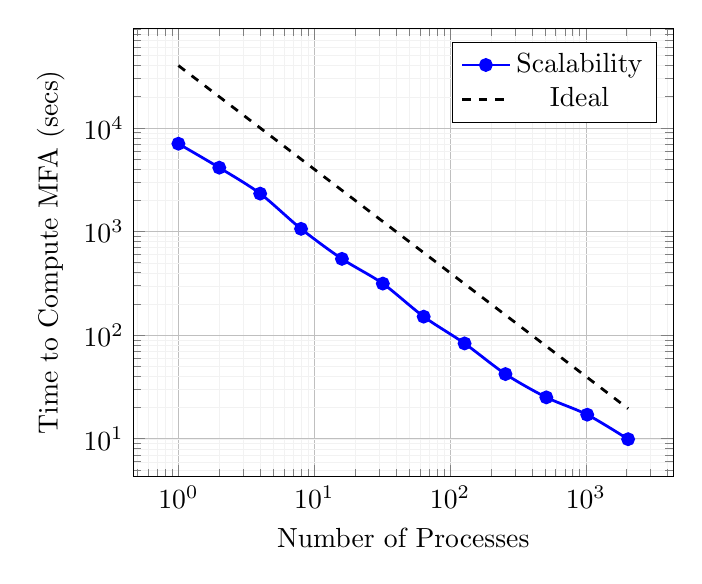
\begin{tikzpicture}
	
	\begin{loglogaxis}[
	legend pos= north east,
%	ymin = 0.0005, ymax = 0.01,
	xlabel=Number of Processes,
	ylabel=Time to Compute MFA (secs),
%	nodes near coords*={\Label},
%	visualization depends on={value \thisrow{label} \as \Label},
	grid=both,
	grid style={line width=.1pt, draw=gray!10},
	major grid style={line width=.2pt,draw=gray!50},
	axis line style={latex-latex},
	every axis plot/.append style={line width=1.0pt},
	%axis lines=middle,
	]
	\axispath\draw
	(7.49165,-10.02171)
	|-  (8.31801,-11.32467)
	node[near start,left] {$\frac{dy}{dx} = -2.58$};
	
	\addplot[smooth,mark=*,blue,width=5pt] table [meta=eff]  {
		x y eff
		1	7045.451504	100
		2	4137.296798	85.14558959
		4	2322.884537	75.82653583
		8	1061.974002	82.92871918
		16	544.925238	80.80754722
		32	314.578249	69.98906001
		64	150.8316872	72.98544611
		128	83.16858159	66.18195096
		256	42.09792775	65.37446476
		512	25.07828297	54.870772
		1024	17.07229925	40.30109616
		2048	9.898160849	34.75556641
%		4096	8.519652482	20.18956686
	};

	\addplot[dashed,black,width=2pt] table [meta=class]  {
	x y class 
	1	40000	100
	2	20000	100
	4	10000	100
	8	5000	100
	16	2500	100
	32	1250	100
	64	625	100
	128	312.5	100
	256	156.25	100
	512	78.125	100
	1024	39.0625	100
	2048	19.53125	100
%	4096	9.765625	100
};
	
	\legend{Scalability\\Ideal\\}
	
	\end{loglogaxis}
	\end{tikzpicture}
	\caption{Strong scalability of the 2-D CESM Problem with 4,096 subdomains and 100 control points/subdomain}
	\label{fig:cesm-strong-scalability}
\end{figure}


%\paragraph{Positioning Figures and Tables} Place figures and tables at the top and 
%``Fig.~\ref{fig}'', even at the beginning of a sentence.

%\begin{table}[htbp]
%\caption{Table Type Styles}
%\begin{center}
%\begin{tabular}{|c|c|c|c|}
%\hline
%\textbf{Table}&\multicolumn{3}{|c|}{\textbf{Table Column Head}} \\
%\cline{2-4} 
%\textbf{Head} & \textbf{\textit{Table column subhead}}& \textbf{\textit{Subhead}}& \textbf{\textit{Subhead}} \\
%\hline
%copy& More table copy$^{\mathrm{a}}$& &  \\
%\hline
%\multicolumn{4}{l}{$^{\mathrm{a}}$Sample of a Table footnote.}
%\end{tabular}
%\label{tab1}
%\end{center}
%\end{table}

%\begin{figure}[htbp]
%\centerline{\includegraphics{fig1.png}}
%\caption{Example of a figure caption.}
%\label{fig}
%\end{figure}


%% Conclusions section
\section{Summary}
\label{sec:conclusions}

%\comment{Future work: extensions to fully adaptive calculations with castelejau knot insertion techniques to match constraints across boundaries, and extensions to \dimension{3}, potential use of hierarchical NURBS bases to accelerate error and parallel solver convergence \cite{schillinger2013}; unstructured datasets and domains}

We have presented a scalable DD approach to tackle the issue of discontinuous B-spline based MFA representations when performing the computations in parallel. The Restricted Additive Schwarz (RAS) method is a natural algorithmic fit for data analysis problems to create efficient MFA solutions in parallel. Through the use of Schwarz-based iterative schemes, combined with constrained local subdomain solvers, the two-level iterative technique has been shown to be robust in converging to the compressed functional representation of the given data, without sacrificing the approximation accuracy measured on a single subdomain of equivalent control point resolution. Replacing B-spline bases with NURBS bases ($W \ne 1$) only requires imposing the constraints on the $\vec{P}_i W_i$ data instead of $\vec{P}_i$ alone, which is naturally accomplished with minor modifications in \algo{alg:pseudocode}. This can also be combined with aposteriori error measures \cite{nashed-rational} to adaptively resolve solution variations while ensuring higher-order continuity across subdomain boundaries with appropriate knot insertion, removal and communication of shared DoFs in $\Delta \cup \delta$ regions. Another natural way to ensure continuity across adaptively resolved NURBS or B-spline patches would be to use T-splines \cite{sederberg-2004}, which are specifically designed for merging higher-dimensional surfaces with non-matching knot locations. All presented ideas should extend for T-splines instead of B-splines as well with modifications to $\mathcal{C}$  in \eqt{eq:global-constrained-problem}.

We have demonstrated that the use of overlap layers $\delta$ can certainly improve the overall MFA accuracy, with a slightly larger one-time setup cost that gets amortized in the overall computation time. We determined that for all the problems tested, including real datasets, $\left| \delta \right|=p$ to $\left| \delta \right|=2p$ is optimal in terms of error recovery and computational cost even for \dimension{3} problems up to 32,768 tasks.
%
%\comment{mention that there are natural extensions to adaptive error resolution with knot insertion and deletion \cite{nashed-rational} and NURBS computation instead of B-splines that are left for future work}
%
%Additionally, the strong scalability of the algorithm was demonstrated for a large \dimension{3} combustion dataset with 209M data points. 
The iterative scheme shows good parallel performance for both \dimension{2} and \dimension{3} problems tested, and the parallel efficiency degrades only when the cost of nearest neighbor subdomain data exchanges start to creep up beyond the cost of the local constrained subdomain solve. Given that scaling characteristics of these processes are well understood in the literature, the parallel speedups behave predictably well at scale on large computing machines tested.
%due to the lack of local computation work in comparison with the latency and communication costs associated with the nearest-neighbor exchanges of constraint data. 


The \texttt{PyDIY} based Python implementations for 1-, 2- and 3-dimensional problems have been shown to resolve large, complex solution profiles with strong gradient variations, even under decreasing subdomain sizes. Depending on the needs for visualization or in-situ analysis, choices on clamped or floating knots can be made with no modifications to the implementation. This scheme can also be used to achieve scalable high-order solution field transfers between component models, a process more generally referred to as {\em remapping} \cite{dukowicz1987accurate}, by imposing constraints on the subdomain solvers to satisfy various metrics of interest \cite{mahadevan2022} such as global conservation and monotonicity. The exploration of parallel MFA for such applications will be pursued in the future.


%The presented RAS-based solver approach can be easily extended to this adaptive case to impose constraints across subdomain patch boundaries, while local constraints within each block 
%%to satisfy hanging node DoFs 
%can be imposed with appropriate T-spline basis modifications.

%Within this infrastructure, we can also utilize a multilevel MFA representation that hierarchically refines the approximation at each level \cite{schillinger2013} by decreasing the number of subdomains used, similar to ideas in standard multilevel methods \cite{brandt1977}. Such computations involving multilevel MFA such as the ones using hierarchical B-splines \cite{bornemann2013} can significantly reduce the computational cost of the local subdomain solvers, which dominate the total computational time. With appropriate choices of prolongation and restriction operators, the iterative scheme can be used with a multilevel subdomain solver to efficiently produce accurate and compact functional approximation of given data, especially in higher dimensions.

%\comment{Another application is as a smoother for datasets with inherent noise; can reference arxiv preprint by David}

%\comment{talk about application to remapping in multiphysics problems and how we can create conservative maps with appropriate constraints imposed on integrals over the domain etc}

%The methodology and experiments presented in the paper are implemented primarily in Python. 
%The current Pythonic interface, PyDIY is only a barebones interface. 
%These algorithms will be ported to the more production-ready C++ MFA codebase \cite{mfa-codebase} in the future. The new implementations will directly make use to the DIY C++ library, and all its features for data decomposition along with fast local subdomain solvers without overheads typically associated with Python codes. We expect that the RAS hierarchical solver implementation in C++ will allow for scalable and efficient application of NURBS-based MFA to much larger problems, without losing solution continuity or approximation accuracy.
%and hence, a better estimate of the overall performance of both the RAS iterative scheme and the subdomain solvers without the overheads of dependent solvers in Python will provide 

%{\color{red} 
	%	it would also be interesting to use multilevel techniques to create a hierarchical MFA representation and use ASM to accelerate finer solves using coarser control point data. Need to explore this idea further but can propose it here as future exploration topic
	%}

%\begin{itemize}
%	\item What did we implement to enhance speedup of the MFA framework and did we preserve accuracy of the underlying method ?
%	\item Did we speedup the actual computation by performing DD with ASM global iterations for some of the problem data ?
%	\item Does the method scale as a function of domains and problem size ? 
%	\item What advantages does it provide for fix-up schemes that can be used in a post-processing step (ref Iulian's blending idea) ?
%	\item Future extensions to T-splines and local adaptivity and potential complications involved
%\end{itemize}


%% acknowledgements section
\section*{Acknowledgments}

This work is supported by Advanced Scientific Computing Research, Office of Science, U.S. Department of Energy, under Contract DE-AC02-06CH11357, program manager Laura Biven. We gratefully acknowledge the computing resources provided on the Theta supercomputer operated by Argonne Leadership Computing Facility, which is a DOE Office of Science User Facility supported under Contract DE-AC02-06CH11357, which was used to generate all the strong and weak scaling results. This research also used resources in the Bebop, a high-performance computing cluster operated by the Laboratory Computing Resource Center (LCRC) at Argonne National Laboratory to test and optimize performance of the drivers at scale.





%\appendix
%\section{An example appendix} 
%\lipsum[71]
%
%\begin{lemma}
%	Test Lemma.
%\end{lemma}


%\pagebreak
\bibliographystyle{siamplain}
\bibliography{asm-mfa}

\pagebreak
\section*{Government License}

The submitted manuscript has been created by UChicago Argonne, LLC, 
Operator of Argonne National Laboratory (“Argonne”). Argonne, a U.S. 
Department of Energy Office of Science laboratory, is operated under 
Contract No. DE-AC02-06CH11357. The U.S. Government retains for itself, and others acting on its behalf, a paid-up nonexclusive, irrevocable 
worldwide license in said article to reproduce, prepare derivative 
works, distribute copies to the public, and perform publicly and display 
publicly, by or on behalf of the Government. The Department of Energy 
will provide public access to these results of federally sponsored 
research in accordance with the \href{http://energy.gov/downloads/doe-public-access-plan}{DOE Public Access Plan}.


\end{document}
